\documentclass{article}


\usepackage[preprint]{neurips_2025}


\usepackage[utf8]{inputenc} % allow utf-8 input
\usepackage[T1]{fontenc}    % use 8-bit T1 fonts
\usepackage{hyperref}       % hyperlinks
\usepackage{url}            % simple URL typesetting
\usepackage{booktabs}       % professional-quality tables
\usepackage{amsfonts}       % blackboard math symbols
\usepackage{nicefrac}       % compact symbols for 1/2, etc.
\usepackage{microtype}      % microtypography
\usepackage{xcolor}         % colors
\usepackage{graphicx}
\usepackage{placeins}
\raggedbottom

% Language setting
% Replace `english' with e.g. `spanish' to change the document language
\usepackage[english]{babel}

\newcommand{\gs}{\mathcal G_s}
\newcommand{\gsc}{\mathcal G_s^C}
\newcommand{\bs}{\mathcal B_s}
\newcommand{\bsc}{\mathcal B_s^C}
\newcommand{\ew}[1]{\hat w_n(#1)}
\newcommand{\prob}[1]{\mathbb{P}\Big(#1\Big)}
\newcommand{\sregret}[2]{\tilde R_{#1,#2}(n)}
\newcommand{\instset}{\mathcal W_{w,\Delta}}
\newcommand{\minmax}{\underset{\phi}{\inf}\,\underset{\bar w}{\sup}\,}

\newcommand{\vct}{\boldsymbol }
\newcommand{\sR}{\mathfrak{R}}

\renewcommand{\hat}{\widehat}
\renewcommand{\tilde}{\widetilde}

 \newcommand{\bF}{\mathbb{F}}
 \newcommand{\bV}{\mathbb{V}}
 \newcommand{\bU}{\mathbb{U}}
 \newcommand{\bW}{\mathbb{W}}
 \newcommand{\bR}{\mathbb{R}}
  \newcommand{\bN}{\mathbb{N}}
   \newcommand{\bE}{\mathbb{E}}
 \newcommand{\bP}{\mathbb{P}}
 \newcommand{\cC}{\mathcal{C}}
 \newcommand{\cS}{\mathcal{S}}
 \newcommand{\cT}{\mathcal{T}}
\newcommand{\cK}{\mathcal{K}}
 \newcommand{\cN}{N}
 \newcommand{\cE}{\mathcal{E}}
 \newcommand{\cD}{\mathcal{D}}
 \newcommand{\cH}{\mathcal{H}}
  \newcommand{\cW}{\mathcal{W}}
\usepackage{amsmath}
\usepackage{amssymb}
\usepackage{amsthm}
\usepackage[table]{xcolor}
\usepackage{multirow}
\usepackage{booktabs}
\usepackage{threeparttable}
\usepackage{tabularx}
%%%%%%%%%%%%%%%%%%%%%%%%%%%%%%%%
% THEOREMS
%%%%%%%%%%%%%%%%%%%%%%%%%%%%%%%%
\theoremstyle{plain}
\newtheorem{theorem}{Theorem}[section]
\newtheorem{proposition}[theorem]{Proposition}
\newtheorem{lemma}[theorem]{Lemma}
\newtheorem{corollary}[theorem]{Corollary}
\newtheorem{remark}[theorem]{Remark}
\theoremstyle{definition}
\newtheorem{definition}[theorem]{Definition}
\newtheorem{assumption}[theorem]{Assumption}
% \theoremstyle{remark}
\usepackage{algorithm} \usepackage{algorithmic}

\hypersetup{
  hidelinks,
  pdftitle={Variance-Gated Discounted Thompson Sampling for Non-Stationary Bandits},
  pdfauthor={Mayand Gulati, Kerong Wang, Wei-Chen Au}
}


\title{Variance-Gated Discounted Thompson Sampling for Non-Stationary Bandits}


% The \author macro works with any number of authors. There are two commands
% used to separate the names and addresses of multiple authors: \And and \AND.
%
% Using \And between authors leaves it to LaTeX to determine where to break the
% lines. Using \AND forces a line break at that point. So, if LaTeX puts 3 of 4
% authors names on the first line, and the last on the second line, try using
% \AND instead of \And before the third author name.


\author{%
  Mayand Gulati, Kerong Wang, Wei-Chen Au \\
  Department of Electrical and Computer Engineering\\
  University of California, Santa Barbara
}


\begin{document}


\maketitle


\begin{abstract}
 We study learning in non-stationary Bernoulli multi-armed bandits, where arm rewards evolve over time without assuming any specific trend. While Thompson Sampling (TS) performs well in stationary settings, it adapts slowly when rewards change. Discounted Thompson Sampling (dTS) improves responsiveness by exponentially forgetting past observations, but a single fixed discount factor creates a tradeoff between fast adaptation and stability. We propose Variance-Gated Discounted Thompson Sampling (VG-dTS), which treats non-stationarity as a latent signal and estimates volatility online from posterior prediction errors to dynamically adjust the discount factor. Experiments on multiple non-stationary environments compare VG-dTS against TS, dTS, dOTS, REXP3, Dynamic TS, and Beta-SWTS. Across the full eight-environment suite, VG-dTS achieves the lowest tuned average normalized regret (0.1047) and the lowest fixed-parameter average normalized regret (0.1351) on the evaluated realizations. These comparisons use unequal tuning grids and do not establish statistical significance or isolate the contribution of each algorithmic component.
\end{abstract}


\section{Introduction}

The multi-armed bandit (MAB) problem studies sequential decision-making under uncertainty, where a learner must balance exploration and exploitation to minimize regret \cite{robbins1952,lai1985}. In stationary settings, both UCB-style methods \cite{auer2002finite,audibert2009,garivier2011klucb} and Thompson Sampling (TS) \cite{thompson1933,agrawal2012analysis,agrawal2013further,russo2018tutorial} are strong and well understood.

Many practical systems are non-stationary: reward distributions drift, switch, or evolve over time. This introduces a core tradeoff between retaining useful history and forgetting stale evidence. Prior work addresses this challenge through switching-bandit analyses \cite{garivier2011switching,hartland2007,besbes2014}, sliding-window estimators \cite{trovo2020}, change-detection mechanisms \cite{liu2018change}, and discounted Bayesian updates such as discounted TS (dTS) \cite{raj2017taming}. A persistent issue is sensitivity to manually chosen forgetting rates.

We propose Variance-Gated Discounted Thompson Sampling (VG-dTS), an adaptive-forgetting variant of TS for non-stationary Bernoulli bandits. VG-dTS estimates arm-wise volatility from standardized posterior prediction errors and maps this signal to time-varying discount factors. A configurable reliability gate can blend a default discount with volatility-driven adaptation when evidence is scarce. A gradual blend requires $n_0>0$; the fixed protocol and seven of eight tuned settings instead use $n_0=0$, which opens the gate fully whenever effective evidence is positive.

Our empirical study evaluates VG-dTS on eight non-stationary environments and compares against strong baselines used throughout this paper: TS, dTS, dOTS, REXP3, Dynamic TS, and Beta-SWTS. Across tuned and fixed-parameter protocols, VG-dTS achieves the lowest average normalized regret on the eight evaluated environment realizations, although other methods lead in several individual environments.

\paragraph{Contributions.}
This paper makes three concrete contributions.
First, we propose VG-dTS: a Thompson-style non-stationary bandit policy that couples prior-preserving discounting with arm-wise volatility gating.
Second, we provide a unified experimental framework over eight environments that span periodic drift, abrupt changes, mixed dynamics, and stochastic switching, and we evaluate under both tuned and fixed-parameter protocols.
Third, we report a lower eight-environment average regret than the evaluated fixed-discount TS variants under both protocols, while documenting the scope and limitations of this comparison.

\section{Related Work}
Non-stationary bandits have been studied through multiple lenses. Foundational analyses characterize switching and variation-budget settings and show the central tradeoff between adaptation and estimation stability \cite{garivier2011switching,hartland2007,besbes2014}. Practical methods include sliding-window estimators \cite{trovo2020}, explicit change-detection approaches \cite{liu2018change}, and discounted Bayesian updates such as dTS \cite{raj2017taming}.
In this paper, we cite change-detection methods as relevant context but do not benchmark them directly; our empirical set focuses on TS-family and adversarial-style baselines used in our implementation pipeline.

Our evaluation compares against baselines that represent these design choices: TS \cite{thompson1933,russo2018tutorial}; dTS, dOTS, and Dynamic TS \cite{raj2017taming}; REXP3 \cite{besbes2014,auer2002nonstochastic}; and Beta-SWTS-style windowed Bayesian estimation \cite{trovo2020}. This mix tests both tuned performance and fixed-parameter robustness across heterogeneous non-stationary regimes.

\subsection{Background: Thompson Sampling}
In Bernoulli bandits with $K$ arms, each arm $k$ has an unknown success probability $\mu_k \in [0,1]$. Thompson Sampling (TS), algorithm \ref{alg:bernts}, maintains a posterior over each $\mu_k$ and, at each round, samples one candidate value per arm, then selects the arm with the highest sampled value \cite{thompson1933,russo2018tutorial}.

Under a Beta--Bernoulli model, TS keeps $\mu_k \sim \mathrm{Beta}(\alpha_k,\beta_k)$ and updates only the played arm after observing reward $R_t \in \{0,1\}$:
\[
(\alpha_{A_t},\beta_{A_t}) \leftarrow (\alpha_{A_t}+R_t,\beta_{A_t}+1-R_t).
\]
This yields a simple exploration--exploitation mechanism: uncertain arms retain wider posteriors (more exploration), while repeatedly successful arms concentrate near higher means (more exploitation). A short conjugacy derivation is provided in Appendix~\ref{app:beta_conjugacy}.

\begin{algorithm}[!htbp]
\caption{\textsc{BernTS}$(K,\alpha,\beta)$ (Beta--Bernoulli Thompson Sampling)}
\label{alg:bernts}
\begin{algorithmic}[1]
\FOR{$t = 1,2,\ldots,T$}
    \FOR{$k = 1,\ldots,K$}
        \STATE Sample $\hat{\mu}_{k} \sim \mathrm{Beta}(\alpha_k,\beta_k)$
    \ENDFOR
    \STATE $A_t \leftarrow \arg\max_{k} \hat{\mu}_{k}$
    \STATE Play arm $A_t$ and observe reward $R_t \in \{0,1\}$
    \STATE $(\alpha_{A_t},\beta_{A_t}) \leftarrow (\alpha_{A_t} + R_t,\ \beta_{A_t} + 1 - R_t)$
\ENDFOR
\end{algorithmic}
\end{algorithm}


\section{Problem Formulation}
We consider a non-stationary multi-armed bandit setup similar to \cite{raj2017taming}.
Let $\cK=[K]$ be the set of arms available to the decision maker, where $[K]$ denotes the set $[K]=\{1,\ldots,K\}$ for any positive integer $K$.
Let the horizon of the game be $T$. For each round $t\in[T]$, the learner chooses an arm $A_t\in\cK$ and observes a Bernoulli reward
$R_t\sim\mathrm{Bernoulli}(\mu_{A_t,t})$, where $\mu_{k,t}\in[0,1]$ denotes arm $k$'s expected reward at time $t$.
At any instant $t$, we say the arm with the highest expected reward is the best arm, and we denote its expected reward by $\mu^*_t = \max_{k \in \cK}\{\mu_{k,t}\}$.

Recall that in stationary settings, for each arm $k$, we have $\mu_{k,t_1}=\mu_{k,t_2}$ for all $t_1,t_2 \in [T]$, so the expected reward of each arm is fixed.
In non-stationary systems, these expected rewards evolve over time. We do not impose a specific parametric trend on this evolution.
Common alternatives in the literature include bounded variation
($\sum_{t=2}^T|\mu_{k,t}-\mu_{k,t-1}| \leq C$), Lipschitz evolution
($|\mu_{k,t}-\mu_{k,s}| \leq L|t-s|$), or latent-state dynamics with limited volatility.
To evaluate robustness without committing to a single assumption family, we benchmark across diverse synthetic environments.

\subsection{Prior Work and Inspirations (dTS and dOTS)}
\cite{raj2017taming} introduced Discounted Thompson Sampling (dTS) that maintains discounted success/failure pseudo-counts $(S_k,F_k)$ per arm and samples
\[
\theta_k \sim \mathrm{Beta}(S_k+\alpha_0,\;F_k+\beta_0),\qquad
A_t=\arg\max_k \theta_k.
\]
After observing Bernoulli reward $R_t\in\{0,1\}$ for played arm $A_t$, dTS applies exponential discounting with factor $\gamma\in(0,1]$:
\[
S_{A_t}\leftarrow \gamma S_{A_t}+R_t,\qquad
F_{A_t}\leftarrow \gamma F_{A_t}+(1-R_t),
\]
and for all unplayed arms $j\neq A_t$,
\[
S_j\leftarrow \gamma S_j,\qquad F_j\leftarrow \gamma F_j.
\]
Note that the ``restless'' discounting feature means all arms are discounted equally, even when not selected.

The authors also propose Discounted Optimistic Thompson Sampling (dOTS), which increases exploitation by clipping each sampled score from below by its posterior mean. More specifically, 
\[
\theta_k^{\mathrm{dOTS}} \triangleq
\max\!\left\{
\theta_k,\;
\frac{S_k+\alpha_0}{S_k+F_k+\alpha_0+\beta_0}
\right\}.
\]
To summarize, dTS introduces global fixed-rate forgetting for non-stationary environments, and dOTS adds optimistic scoring on top of dTS.


\section{Variance-Gated Discounted Thompson Sampling (VG-dTS)}

\subsection{From discounted TS to volatility-gated discounting}
Discounted Thompson Sampling (dTS) \cite{raj2017taming} addresses non-stationarity by \emph{forgetting} old evidence: posterior parameters are shrunk toward a base prior so that recent observations dominate decisions.
In a Beta--Bernoulli model, we represent arm $k$'s belief by $\mu_{k}\sim \mathrm{Beta}(\alpha_k,\beta_k)$, where $\alpha_k-1$ and $\beta_k-1$ can be interpreted as (possibly fractional) pseudo-counts of past successes and failures.
A \emph{prior-preserving discount} step with discount factor $\gamma\in(0,1]$ is
\begin{equation}
\alpha_k \leftarrow 1+\gamma(\alpha_k-1),\qquad
\beta_k \leftarrow 1+\gamma(\beta_k-1).
\label{eq:prior_preserving_discount}
\end{equation}
This transformation leaves the uniform prior $\mathrm{Beta}(1,1)$ unchanged and scales the effective evidence $(\alpha_k+\beta_k-2)$ by exactly $\gamma$ before the reward update.
Intuitively, smaller $\gamma$ means faster forgetting and quicker adaptation, but also higher estimation variance.

A core limitation of fixed-$\gamma$ methods is that the ``right'' forgetting rate depends on \emph{both} the environment dynamics and the amount of data collected:
when the arm behavior is stable, aggressive forgetting wastes information; when the arm changes rapidly, conservative forgetting reacts too slowly.
Therefore, we propose VG-dTS (Algorithm \ref{alg:vgdts}). It replaces the single global $\gamma$ by \emph{arm-wise, time-varying} discounts $\gamma_{k,t}$ driven by an online estimate of non-stationarity.

\subsection{Standardized surprise as a change signal}
At round $t$, VG-dTS forms a Thompson sample for each arm. All reported VG-dTS experiments select $A_t$ using the optimistic score $\max\{\widetilde{\mu}_{k,t},\bar{\mu}_{k,t}\}$, rather than the sample alone.
Let $\bar{\mu}_{k,t}$ denote the current posterior mean,
$
\bar{\mu}_{k,t} \triangleq \frac{\alpha_k}{\alpha_k+\beta_k},
$
computed \emph{before} incorporating the round-$t$ observation.
After playing $A_t$, we observe a Bernoulli reward $R_t\in\{0,1\}$.
In all experiments in this paper, we use $x_t=R_t$.
(Optionally, one may replace $R_t$ by a real-valued observation $x_t$ as a \emph{reward proxy}.)

We define a \emph{standardized surprise} (a normalized prediction error) for the played arm.
Let $b\in\{0,1\}$ be a one-sided flag:
\begin{equation}
e_t^{(b)}
\triangleq
\begin{cases}
|x_t-\bar{\mu}_{A_t,t}|, & b=0 \quad \text{(two-sided)},\\
\max\{\bar{\mu}_{A_t,t}-x_t,0\}, & b=1 \quad \text{(downside-only)}.
\end{cases}
\label{eq:surprise_num_main}
\end{equation}
Then
\begin{equation}
s_t
\triangleq
\mathrm{clip}\!\left(
\frac{e_t^{(b)}}
{\sqrt{\max\{\bar{\mu}_{A_t,t}(1-\bar{\mu}_{A_t,t}),\,\epsilon\}}},
\,0,\,c
\right),
\label{eq:surprise_main}
\end{equation}
where $\mathrm{clip}(z,a,b)=\min\{\max\{z,a\},b\}$, $\epsilon>0$ prevents division by very small variances, and $c>0$ caps extreme outliers.
The normalization by $\sqrt{\bar{\mu}(1-\bar{\mu})}$ is crucial: the same absolute error $|x-\bar{\mu}|$ should be considered \emph{more surprising} when the posterior predicts near-certain outcomes (e.g., $\bar{\mu}\approx 0.99$) than when it predicts highly noisy outcomes (e.g., $\bar{\mu}\approx 0.5$).
Thus, $s_t$ measures deviations in ``units of expected noise''.

To translate surprise into an arm-wise non-stationarity signal, VG-dTS maintains for each arm $k$ two exponentially weighted moving average (EWMA) state variables:
a mean-like statistic $m_k$ and a variance-like statistic $v_k$.
Only the played arm is updated (bandit feedback). We use the update order implemented in code: first update $m_k$, then update $v_k$ using the new mean:
\begin{equation}
\widetilde{m}_{A_t} \leftarrow \lambda m_{A_t} + (1-\lambda)s_t,
\qquad
v_{A_t} \leftarrow \lambda v_{A_t} + (1-\lambda)\bigl(s_t-\widetilde{m}_{A_t}\bigr)^2,
\qquad
m_{A_t}\leftarrow \widetilde{m}_{A_t},
\label{eq:ewma_update_main}
\end{equation}
with smoothing parameter $\lambda\in[0,1)$.
We then define the \emph{volatility proxy} for each arm as
\begin{equation}
\nu_{k,t} \triangleq \sqrt{\max\{v_k,0\}}.
\label{eq:vol_proxy_main}
\end{equation}
This proxy measures variation around the EWMA surprise mean, not the magnitude of that mean. Fluctuating surprises can increase $\nu_{k,t}$, whereas a constant large surprise eventually has vanishing centered variation. It is an indirect signal of change, not a calibrated estimate of changes in the true reward mean.

\subsection{Mapping volatility to a discount candidate}
VG-dTS converts $\nu_{k,t}$ into a discount candidate $\gamma^{\mathrm{vol}}_{k,t}\in[\gamma_{\min},\gamma_{\max}]$ with the monotonic principle such that higher volatility $\nu_{k,t}$ will lead to smaller discount factor $\gamma^{\mathrm{vol}}_{k,t}$, so we obtain faster forgetting.

We implement this map in two simple, interpretable families (Appendix~\ref{app:vgdts}):
(i) an inverse-linear map between user-specified low/high volatility levels, and
(ii) a logistic (smooth threshold) map controlled by a midpoint and slope.
These are design choices rather than identities: they enforce boundedness, monotonicity, and numerical stability, while offering clear tuning knobs. All reported experiments use the inverse-linear map; the logistic map is implemented but is not evaluated here.

\subsection{Reliability gate via effective sample size}
Early in learning, volatility estimates are unreliable because the posterior itself is uncertain and each arm may have very few observations.
To temper adaptation when effective evidence is small, VG-dTS can mix the volatility-based discount with a default $\gamma_{\mathrm{def}}$ using a data-dependent gate. The implementation first clips the supplied default to $[\gamma_{\min},\gamma_{\max}]$; throughout the update equations, $\gamma_{\mathrm{def}}$ denotes this clipped value:
\begin{equation}
n^{\mathrm{eff}}_{k,t} \triangleq \max\{\alpha_k+\beta_k-2,\,0\},\qquad
w_{k,t}\triangleq
\begin{cases}
\frac{n^{\mathrm{eff}}_{k,t}}{n^{\mathrm{eff}}_{k,t}+n_0}, & n_0>0,\\
\mathbb{I}\{n^{\mathrm{eff}}_{k,t}>0\}, & n_0=0,
\end{cases}
\label{eq:gate_main}
\end{equation}
where $n^{\mathrm{eff}}_{k,t}$ is the \emph{effective sample size} (pseudo-counts of evidence) and $n_0\ge 0$ is a gate scale.
For $n_0>0$, when $n^{\mathrm{eff}}_{k,t}\ll n_0$, we have $w_{k,t}\approx 0$ and the algorithm relies on $\gamma_{\mathrm{def}}$; when $n^{\mathrm{eff}}_{k,t}\gg n_0$, $w_{k,t}\approx 1$. For $n_0=0$, this is a binary gate: it equals one whenever effective evidence is positive and does not provide a gradual reliability transition.
The final discount is the convex combination
\begin{equation}
\gamma_{k,t} \triangleq (1-w_{k,t})\gamma_{\mathrm{def}} + w_{k,t}\gamma^{\mathrm{vol}}_{k,t},
\qquad
\gamma_{k,t}\in[\gamma_{\min},\gamma_{\max}].
\label{eq:gamma_mix_main}
\end{equation}

\subsection{Full VG-dTS update}
After computing $\gamma_{k,t}$ for all arms, VG-dTS applies the prior-preserving restless discount \eqref{eq:prior_preserving_discount} to \emph{all} arms (reflecting the possibility that any arm may drift), and then performs the standard conjugate update on the played arm:
\begin{equation}
\alpha_{A_t}\leftarrow \alpha_{A_t}+R_t,\qquad
\beta_{A_t}\leftarrow \beta_{A_t}+1-R_t.
\label{eq:conjugate_update_main}
\end{equation}
Similar to \cite{raj2017taming}, we use the optimistic score $\theta_{k,t}=\max\{\widetilde{\mu}_{k,t},\bar{\mu}_{k,t}\}$ in every reported VG-dTS configuration, including the negative control. Standard scoring is supported by the code but is not part of the reported comparison.
\paragraph{What optimism means here}
In standard Thompson scoring, the action score is the posterior sample $\widetilde{\mu}_{k,t}$.
Under optimistic scoring, we instead use
\[
\theta_{k,t}=
\begin{cases}
\widetilde{\mu}_{k,t}, & \text{standard score},\\
\max\{\widetilde{\mu}_{k,t},\bar{\mu}_{k,t}\}, & \text{optimistic score},
\end{cases}
\]
where $\bar{\mu}_{k,t}$ is the posterior mean.
This is a lightweight optimism-in-the-face-of-uncertainty mechanism: it clips overly pessimistic draws upward to the arm's current mean estimate, so arms are less likely to be discarded due to one unlucky sample.
This changes the action-selection distribution. The reported experiments do not include an optimism ablation, so they do not isolate its effect from that of adaptive discounting.

\subsection{Subroutines and intuition}
Algorithm~\ref{alg:vgdts} calls two subroutines:
\texttt{StdSurprise} (Algo.~\ref{alg:apx_stdsurprise}) and \texttt{MapToDiscount} (Algo.~\ref{alg:apx_maptodiscount}).

\texttt{StdSurprise}.
This routine converts an observation into a \emph{dimensionless} prediction error by dividing by the posterior-predicted noise scale.
Flag $b$ selects either two-sided ($b=0$) or downside-only ($b=1$) surprise.
Clipping prevents numerical blow-ups (when $\bar{\mu}(1-\bar{\mu})$ is tiny) and limits the impact of outliers.

\texttt{MapToDiscount}.
This routine enforces the policy decision ``unstable $\Rightarrow$ forget faster'' by mapping $\nu$ to a bounded $\gamma^{\mathrm{vol}}$.
The inverse-linear map is a simple piecewise-linear schedule; the logistic map provides a smooth transition around a midpoint (useful when one believes there is a regime change threshold). More details can be found in Appendix~\ref{app:vgdts}.

\subsection{Basic properties}
VG-dTS satisfies several immediate properties useful for interpretation and implementation.
\begin{itemize}
\item \textbf{Boundedness.} With both $\gamma^{\mathrm{vol}}_{k,t}$ and the clipped $\gamma_{\mathrm{def}}$ in $[\gamma_{\min},\gamma_{\max}]$, and $w_{k,t}\in[0,1]$, their convex combination remains in this interval.
\item \textbf{Monotonicity in volatility.} Both supported maps are nonincreasing in $\nu$. At a fixed gate weight, increasing the proxy cannot increase the final discount.
\item \textbf{Gate behavior.} For $n_0>0$, $w_{k,t}\to 0$ as $n^{\mathrm{eff}}_{k,t}\to 0$ and $w_{k,t}\to 1$ as $n^{\mathrm{eff}}_{k,t}\to\infty$; for $n_0=0$, the implementation uses $w_{k,t}=\mathbb{I}\{n^{\mathrm{eff}}_{k,t}>0\}$.
\item \textbf{Per-round cost.} The method is $O(K)$ per round and stores $O(K)$ state.
\end{itemize}



% \subsection{From Discounted TS to Volatility-Gated dTS}
% Discounted Thompson Sampling (dTS) improves adaptation in non-stationary environments by exponentially forgetting old evidence.
% However, using one fixed discount factor for all arms and all times is fundamentally brittle: a large discount reacts quickly but increases variance, while a small discount is stable but slow after changepoints.
% Our development of VG-dTS started from this mismatch.

% The key idea is to treat non-stationarity as a latent, time-varying signal and estimate it online from posterior prediction errors.
% For the selected arm $A_t$, let $\bar{\mu}_{A_t,t}$ be the current posterior mean and let $x_t$ be the observed binary reward (or reward proxy).
% We compute a standardized surprise signal
% \begin{equation}
% s_t
% =
% \mathrm{clip}\!\left(
% \frac{|x_t-\bar{\mu}_{A_t,t}|}
% {\sqrt{\max\{\bar{\mu}_{A_t,t}(1-\bar{\mu}_{A_t,t}),\epsilon\}}},
% 0,c
% \right),
% \end{equation}
% where $\mathrm{clip}(x,a,b)=\min(\max(x,a),b)$.
% This follows the same estimation-theoretic intuition as normalized innovations: deviations are measured relative to expected uncertainty.
% An EWMA variance of this surprise provides an arm-wise volatility proxy $\nu_{k,t}$.

% VG-dTS then maps volatility to a discount candidate $\gamma^{\mathrm{vol}}_{k,t} \in [\gamma_{\min},\gamma_{\max}]$, with higher volatility implying faster forgetting (smaller $\gamma$).
% To prevent early-round overreaction, we use a volatility gate:
% \begin{equation}
% w_{k,t}=\frac{n^{\mathrm{eff}}_{k,t}}{n^{\mathrm{eff}}_{k,t}+n_0},\qquad
% \gamma_{k,t}=(1-w_{k,t})\gamma_{\mathrm{def}}+w_{k,t}\gamma^{\mathrm{vol}}_{k,t}.
% \end{equation}
% When data are scarce, the algorithm stays near a conservative default discount; as evidence accumulates, it transitions to volatility-driven adaptation.
% In Algorithm~\ref{alg:vgdts}, $s_t$ is the standardized surprise, $(m_k,v_k)$ are EWMA state variables used to estimate volatility, $\nu_{k,t}=\sqrt{v_k}$ is the volatility proxy, and $\gamma^{\mathrm{vol}}_{k,t}$ is the mapped discount candidate. The gate parameter $n_0$ controls how quickly $w_{k,t}$ moves from near $0$ (default discount) to near $1$ (volatility-driven discount) as effective sample size $n^{\mathrm{eff}}_{k,t}$ grows.
% Finally, we optionally apply an optimistic score
% $\theta_{k,t}=\max\{\widetilde{\mu}_{k,t},\bar{\mu}_{k,t}\}$,
% which reduced under-exploration in our fast-changing regimes.

\begin{algorithm}[t]
\caption{\textsc{VG-dTS}: Variance-Gated Discounted Thompson Sampling (reported optimistic configuration)}
\label{alg:vgdts}
\begin{algorithmic}[1]
\STATE \textbf{Input:} $K$, $T$, prior $(\alpha_0,\beta_0)=(1,1)$; bounds $(\gamma_{\min},\gamma_{\max})$; default $\gamma_{\mathrm{def}}$;
EWMA $\lambda$; surprise params $(\epsilon,c,b)$; gate $n_0$; mapping params for \texttt{MapToDiscount}
\STATE $\gamma_{\mathrm{def}}\leftarrow\mathrm{clip}(\gamma_{\mathrm{def}},\gamma_{\min},\gamma_{\max})$
\STATE Initialize $(\alpha_k,\beta_k)\leftarrow(\alpha_0,\beta_0)$ and $(m_k,v_k)\leftarrow(0,0)$ for all $k\in[K]$
\FOR{$t=1,\ldots,T$}
    \FOR{$k=1,\ldots,K$}
        \STATE Sample $\widetilde{\mu}_{k,t}\sim \mathrm{Beta}(\alpha_k,\beta_k)$ and set $\bar{\mu}_{k,t}\leftarrow \frac{\alpha_k}{\alpha_k+\beta_k}$
        \STATE Score $\theta_{k,t}\leftarrow \max\{\widetilde{\mu}_{k,t},\bar{\mu}_{k,t}\}$ \hfill (used in all reported runs)
    \ENDFOR
    \STATE Play $A_t\leftarrow\arg\max_k \theta_{k,t}$ and observe $R_t\in\{0,1\}$; set $x_t\leftarrow R_t$ \hfill (Bernoulli case)
    \STATE $s_t\leftarrow \texttt{StdSurprise}(x_t,\bar{\mu}_{A_t,t};\epsilon,c,b)$
    \STATE Update played-arm EWMA stats $(m_{A_t},v_{A_t})$ using $s_t$ and $\lambda$
    \FOR{$k=1,\ldots,K$}
        \STATE $\nu_{k,t}\leftarrow\sqrt{\max\{v_k,0\}}$ \hfill (volatility proxy)
        \STATE $\gamma^{\mathrm{vol}}_{k,t}\leftarrow \texttt{MapToDiscount}(\nu_{k,t};\gamma_{\min},\gamma_{\max})$
        \STATE $n^{\mathrm{eff}}_{k,t}\leftarrow \max\{\alpha_k+\beta_k-2,0\}$
        \IF{$n_0=0$}
            \STATE $w_{k,t}\leftarrow \mathbb{I}\{n^{\mathrm{eff}}_{k,t}>0\}$
        \ELSE
            \STATE $w_{k,t}\leftarrow \frac{n^{\mathrm{eff}}_{k,t}}{n^{\mathrm{eff}}_{k,t}+n_0}$
        \ENDIF
        \STATE $\gamma_{k,t}\leftarrow (1-w_{k,t})\gamma_{\mathrm{def}} + w_{k,t}\gamma^{\mathrm{vol}}_{k,t}$
        \STATE $\alpha_k\leftarrow 1+\gamma_{k,t}(\alpha_k-1)$;\quad
        $\beta_k\leftarrow 1+\gamma_{k,t}(\beta_k-1)$ \hfill (prior-preserving discount)
    \ENDFOR
    \STATE $\alpha_{A_t}\leftarrow \alpha_{A_t}+R_t$;\quad
    $\beta_{A_t}\leftarrow \beta_{A_t}+1-R_t$ \hfill (conjugate update)
\ENDFOR
\end{algorithmic}
\end{algorithm}

\section{Experiments}
\subsection{Experimental Setup}
We evaluate VG-dTS on Bernoulli non-stationary bandits with horizon $T=5000$ and $K=4$ arms.
All comparisons report \emph{final normalized regret} (lower is better) against strong baselines:
TS \cite{thompson1933,russo2018tutorial}, dTS/dOTS/Dynamic TS \cite{raj2017taming}, REXP3 \cite{besbes2014,auer2002nonstochastic}, and Beta-SWTS-style windowed TS \cite{trovo2020}.
We report two complementary protocols:
\textbf{(i)} tuned-per-environment performance and
\textbf{(ii)} fixed-parameter robustness across environments.

For a single run, we define normalized regret at round $t$ as
\begin{equation}
\mathrm{NR}_t
\triangleq
\frac{1}{t}\sum_{s=1}^{t}\bigl(\mu_s^\star-R_s\bigr)
=
\frac{\sum_{s=1}^{t}\mu_s^\star-\sum_{s=1}^{t}R_s}{t},
\label{eq:nr_def}
\end{equation}
where $\mu_s^\star=\max_k\mu_{k,s}$ is the dynamic-oracle mean and $R_s\in\{0,1\}$ is the realized reward.
This realized statistic may be negative on an individual rollout and is not clipped. Conditional on the fixed environment means, its expectation over both policy randomization and reward noise satisfies
\[
\mathbb{E}[\mathrm{NR}_t]
=
\frac{1}{t}\sum_{s=1}^{t}\bigl(\mu_s^\star-\mathbb{E}[\mu_{A_s,s}]\bigr).
\]
The primary scalar metric is \emph{final normalized regret} $\mathrm{NR}_T$.
Reported values are Monte Carlo averages over repeated rollouts,
\begin{equation}
\widehat{\mathrm{NR}}_T
\triangleq
\frac{1}{N}\sum_{i=1}^{N}\mathrm{NR}^{(i)}_T.
\label{eq:nr_mc}
\end{equation}

Each environment has one fixed mean trajectory, shared by all methods. Rollouts repeat reward and policy randomness, not the environment realization. Within a policy--environment pair, tuning and evaluation use separate pseudo-random seed streams. The legacy arithmetic seed schedule reuses some streams across different pairs, so the cells of the benchmark are not globally independent. Suite averages weight the eight environments equally.

\paragraph{Reproduction settings and provenance.}
The reconstruction uses base seed 0, 70 rollouts per tuning candidate, and $N=1000$ evaluation rollouts at each selected or fixed setting. The original summaries retain parameters and final regrets but not the original invocation or run metadata; these run settings were reconstructed, not recovered from an original log. Evaluation replay at the archived settings reproduced all 119 reported final regrets exactly (two $8\times7$ suites and one seven-method negative control). This validates the evaluation replay, not a fresh hyperparameter search: the full 70-rollout tuning sweep has not been rerun. NumPy 1.26.4 is required to reproduce the archived random-breakpoint realization. The repository's reproduction guide records the seed schedule, dependency versions, commands, and validation scope.

\paragraph{Implemented Dynamic TS baseline.}
Dynamic TS samples from each arm's Beta posterior and updates only the played arm. Before adding the current reward, if that arm's posterior mass $\alpha_{A_t}+\beta_{A_t}$ exceeds $C$, both parameters are multiplied by $C/(C+1)$. This is thresholded discounting of the played arm, including its prior mass; it is not an explicit changepoint test or a hard reset of posteriors.

\subsection{Environment Suite}
Our suite spans smooth drift, abrupt shifts, and mixed/randomized dynamics:
\texttt{slow}, \texttt{fast}, \texttt{abrupt}, \texttt{mixed}, \texttt{random\_breakpoints}, \texttt{random\_drift}, \texttt{global\_switching}, and \texttt{per\_arm\_switching}.
All environments use $T=5000$ and $K=4$ arms, with Bernoulli means clipped to $[0,1]$.
Figure~\ref{fig:env_oracle_gallery} visualizes all eight mean trajectories and their dynamic oracle.
Table~\ref{tab:env_suite_summary} provides a parameter-level summary of this suite.
\begin{table}[H]
\centering
\small
\setlength{\tabcolsep}{4pt}
\begin{tabularx}{\linewidth}{lX}
\toprule
Environment & Dynamics specification used in this paper \\
\midrule
\texttt{slow} & Sinusoidal means $\mu_{k,t}=0.5+0.5\sin(2\pi t/1000+\phi_k)$ with phases $\phi_k\in\{0,\pi/2,\pi,3\pi/2\}$. \\
\texttt{fast} & Same sinusoidal construction as \texttt{slow}, but with period $100$ instead of $1000$. \\
\texttt{abrupt} & Repeating 250-round cycle. All arms start at zero; arm $k$ jumps to level $[0.10,0.37,0.63,0.90]_k$ at zero-based cycle offset $[50,100,150,200]_k$ and stays there until all arms reset to zero. \\
\texttt{mixed} & Arm 1 stationary at $0.65$, arm 2 linear drift ($0.20\rightarrow0.85$), arm 3 bursty ($p_{\text{burst}}=0.05$), arm 4 random two-level switching. \\
\texttt{random\_breakpoints} & Per-arm piecewise-constant means with random breakpoints (4--16), minimum segment length $33$, and minimum jump $0.10$. \\
\texttt{random\_drift} & Randomized sinusoid per arm with amplitude random walk in $[0.05,0.30]$ plus slow drift. \\
\texttt{global\_switching} & With probability $0.02$ per round, all arm means redraw jointly from $\mathrm{Uniform}(0.05,0.95)$. \\
\texttt{per\_arm\_switching} & With probability $0.02$ per arm per round, only that arm redraws from $\mathrm{Uniform}(0.05,0.95)$. \\
\bottomrule
\end{tabularx}
\caption{Specification of the eight benchmark environments.}
\label{tab:env_suite_summary}
\end{table}

\vspace{-2mm}
For each environment, the dynamic oracle at round $t$ is
$k_t^\star=\arg\max_{k\in[K]}\mu_{k,t}$ and its instantaneous expected reward is
$\mu_t^\star=\max_{k\in[K]}\mu_{k,t}$.
The oracle curves in Figure~\ref{fig:env_oracle_gallery} define the reference policy used in normalized-regret computation.

\vspace{-1mm}
\begin{figure}[H]
\centering
\begin{minipage}[t]{0.49\textwidth}
\centering
\textbf{slow}\par\vspace{1mm}
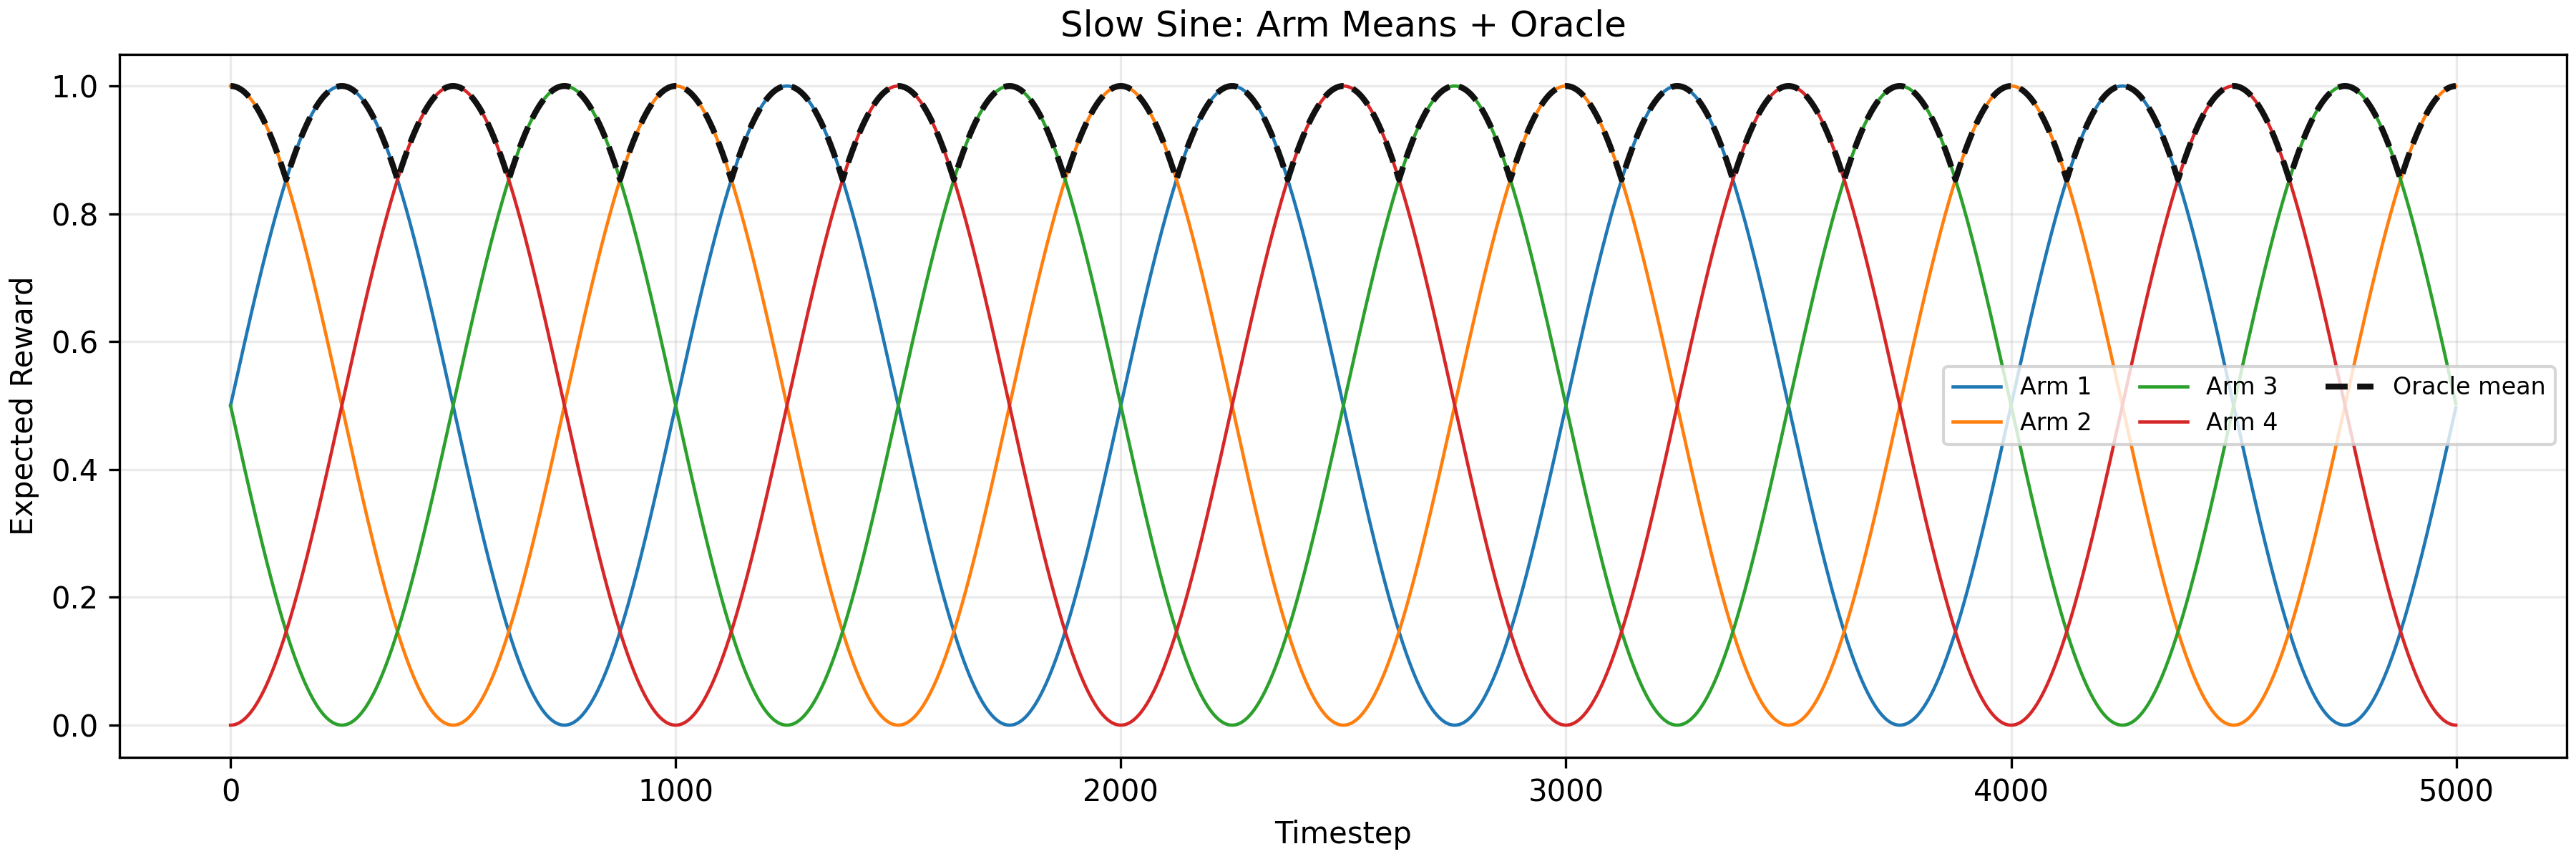
\includegraphics[width=\linewidth]{environment_oracle/environment_oracle_slow.png}
\end{minipage}\hfill
\begin{minipage}[t]{0.49\textwidth}
\centering
\textbf{fast}\par\vspace{1mm}
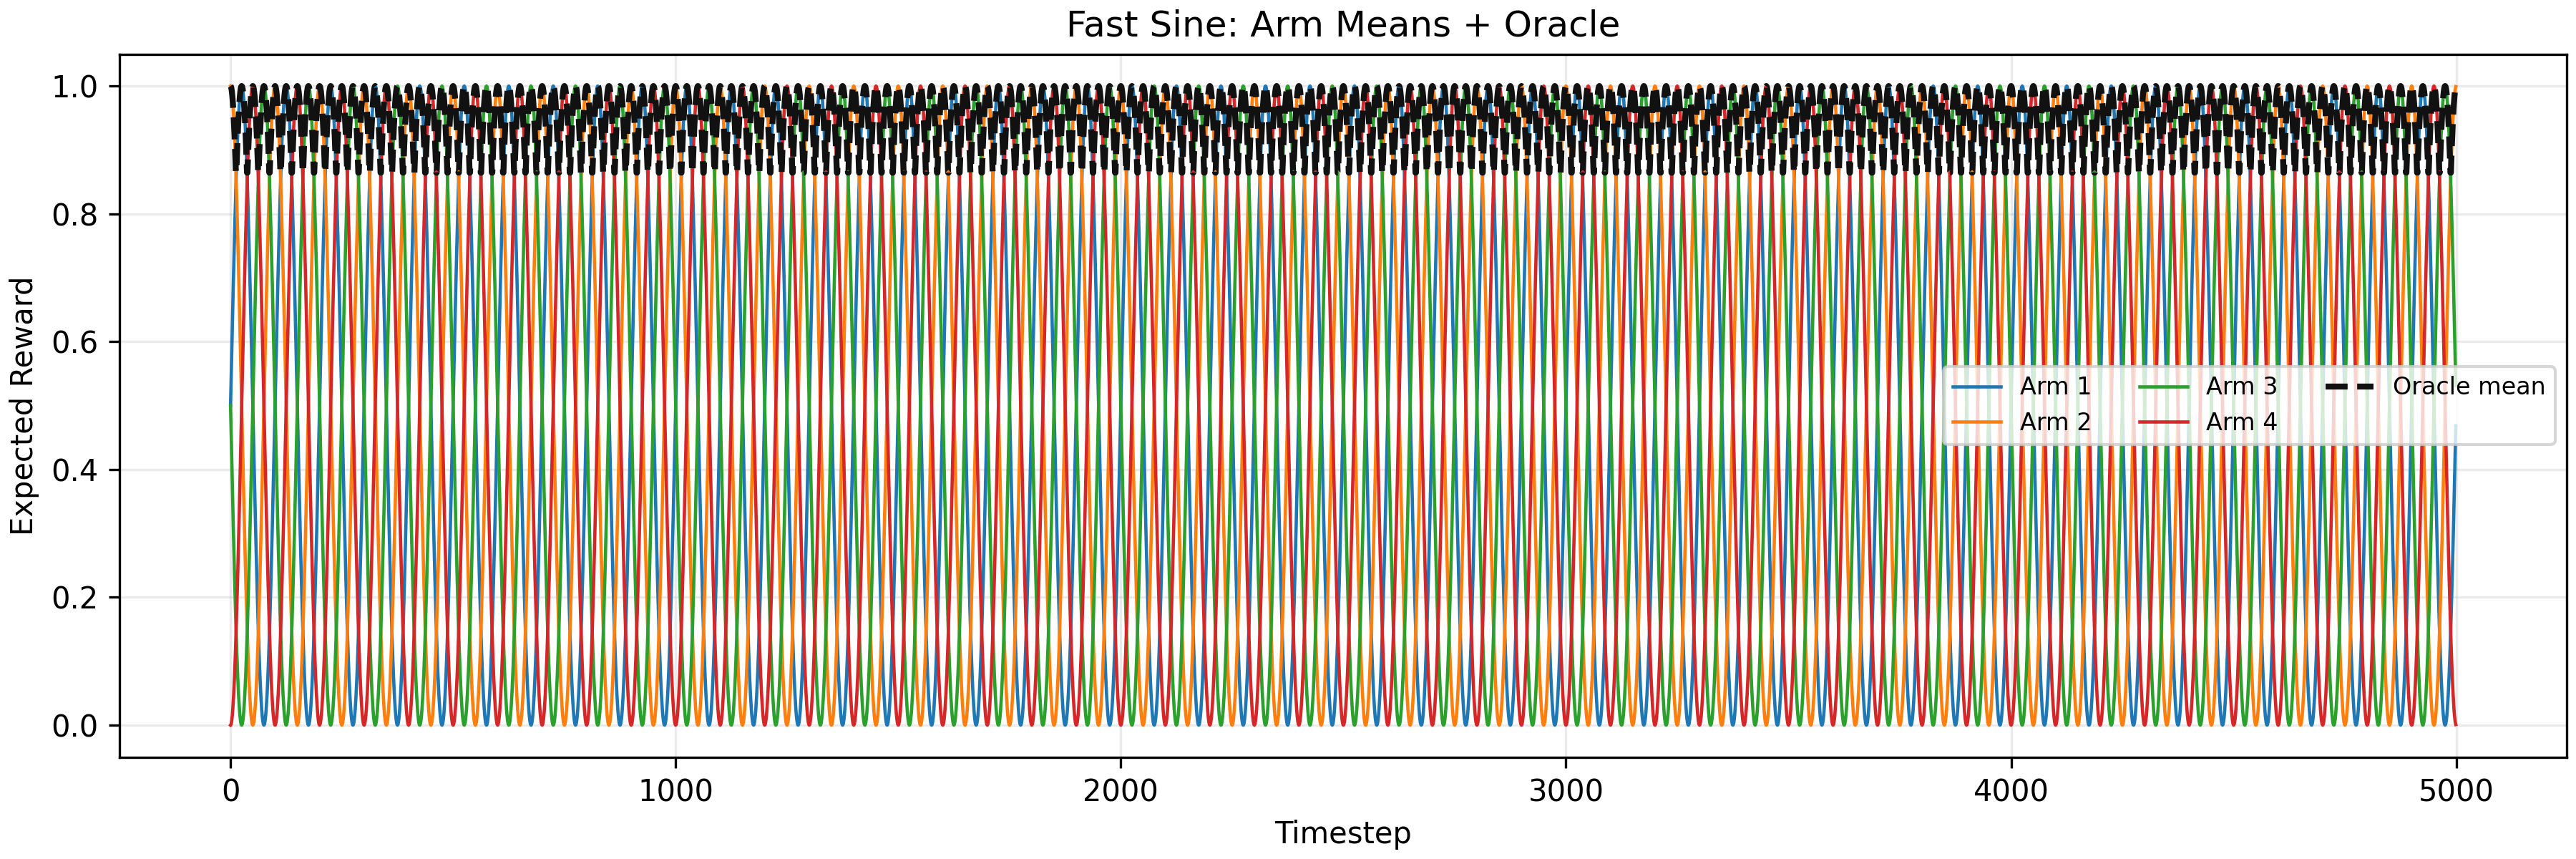
\includegraphics[width=\linewidth]{environment_oracle/environment_oracle_fast.png}
\end{minipage}

\vspace{2mm}
\begin{minipage}[t]{0.49\textwidth}
\centering
\textbf{abrupt}\par\vspace{1mm}
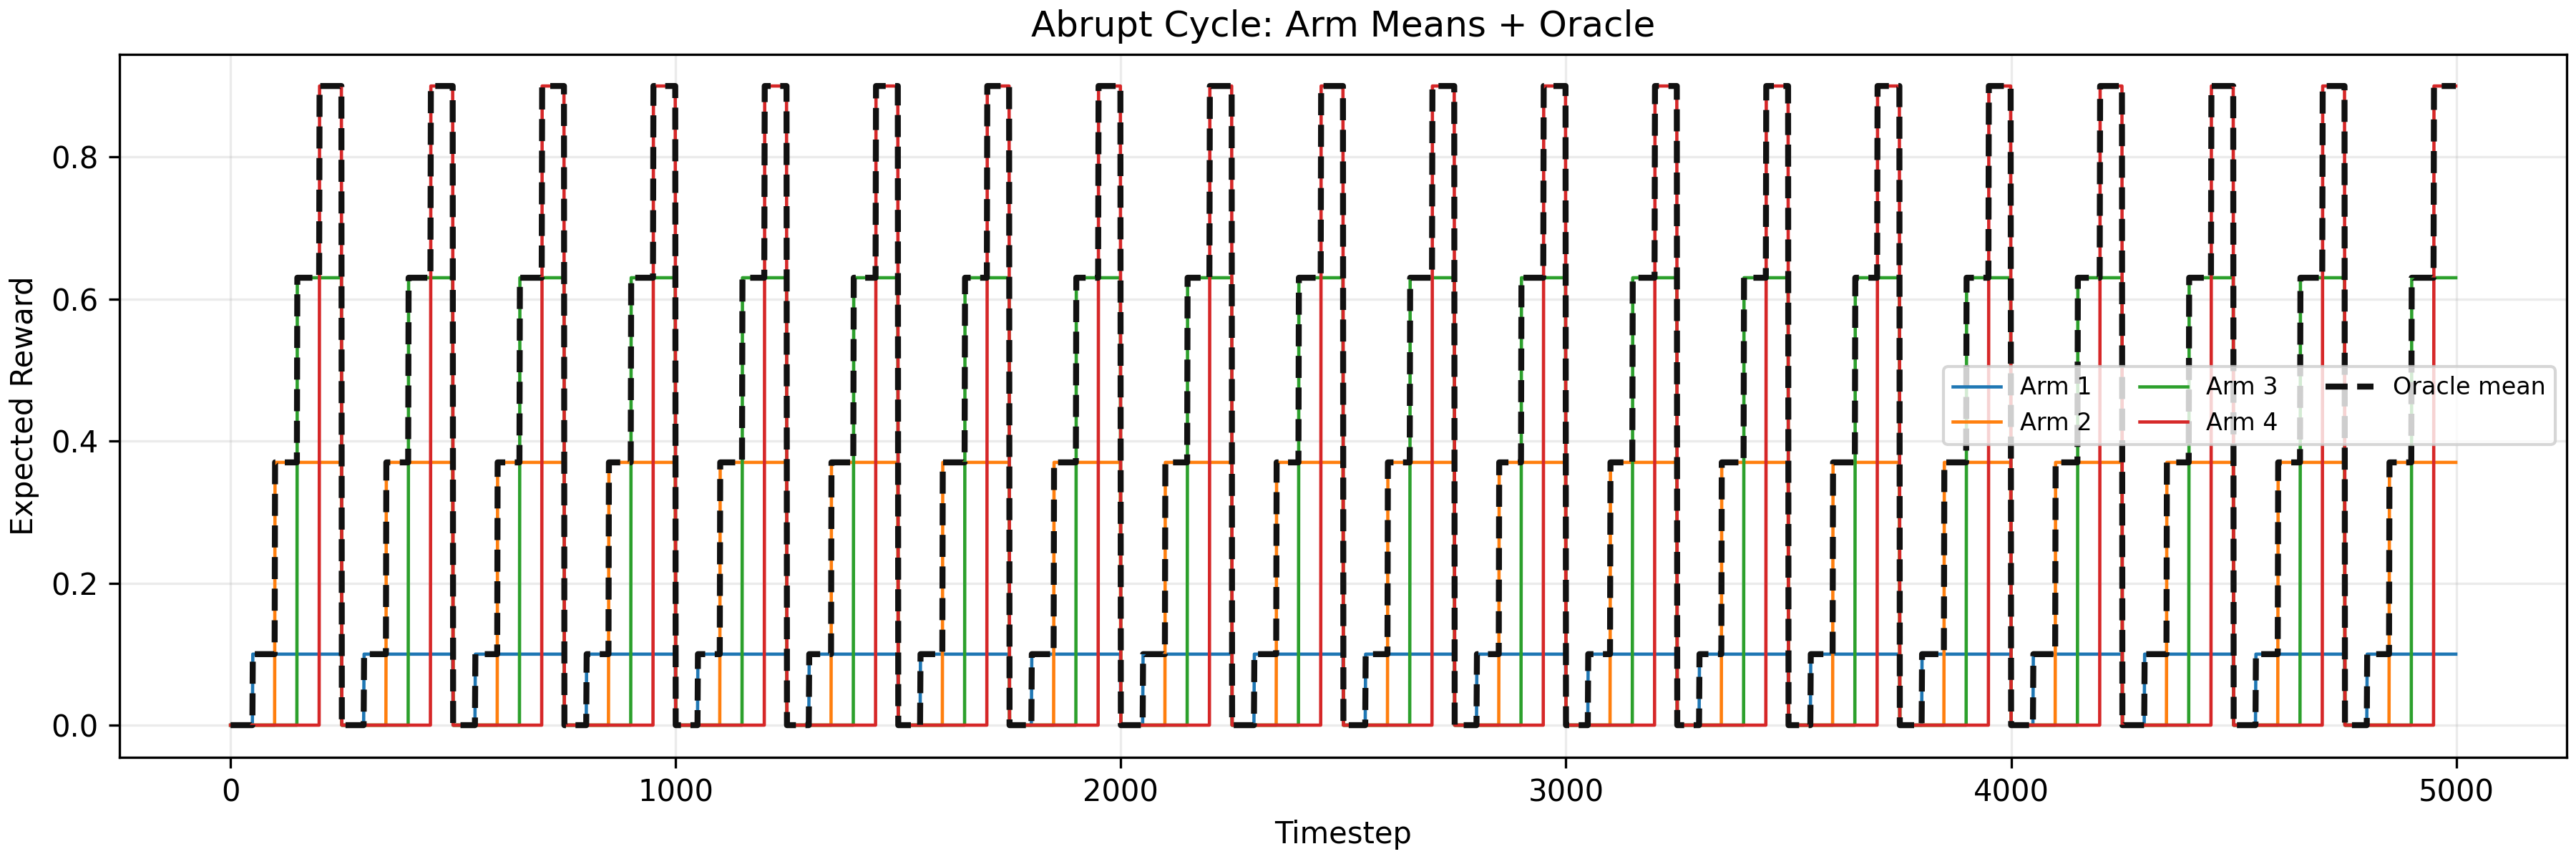
\includegraphics[width=\linewidth]{environment_oracle/environment_oracle_abrupt.png}
\end{minipage}\hfill
\begin{minipage}[t]{0.49\textwidth}
\centering
\textbf{mixed}\par\vspace{1mm}
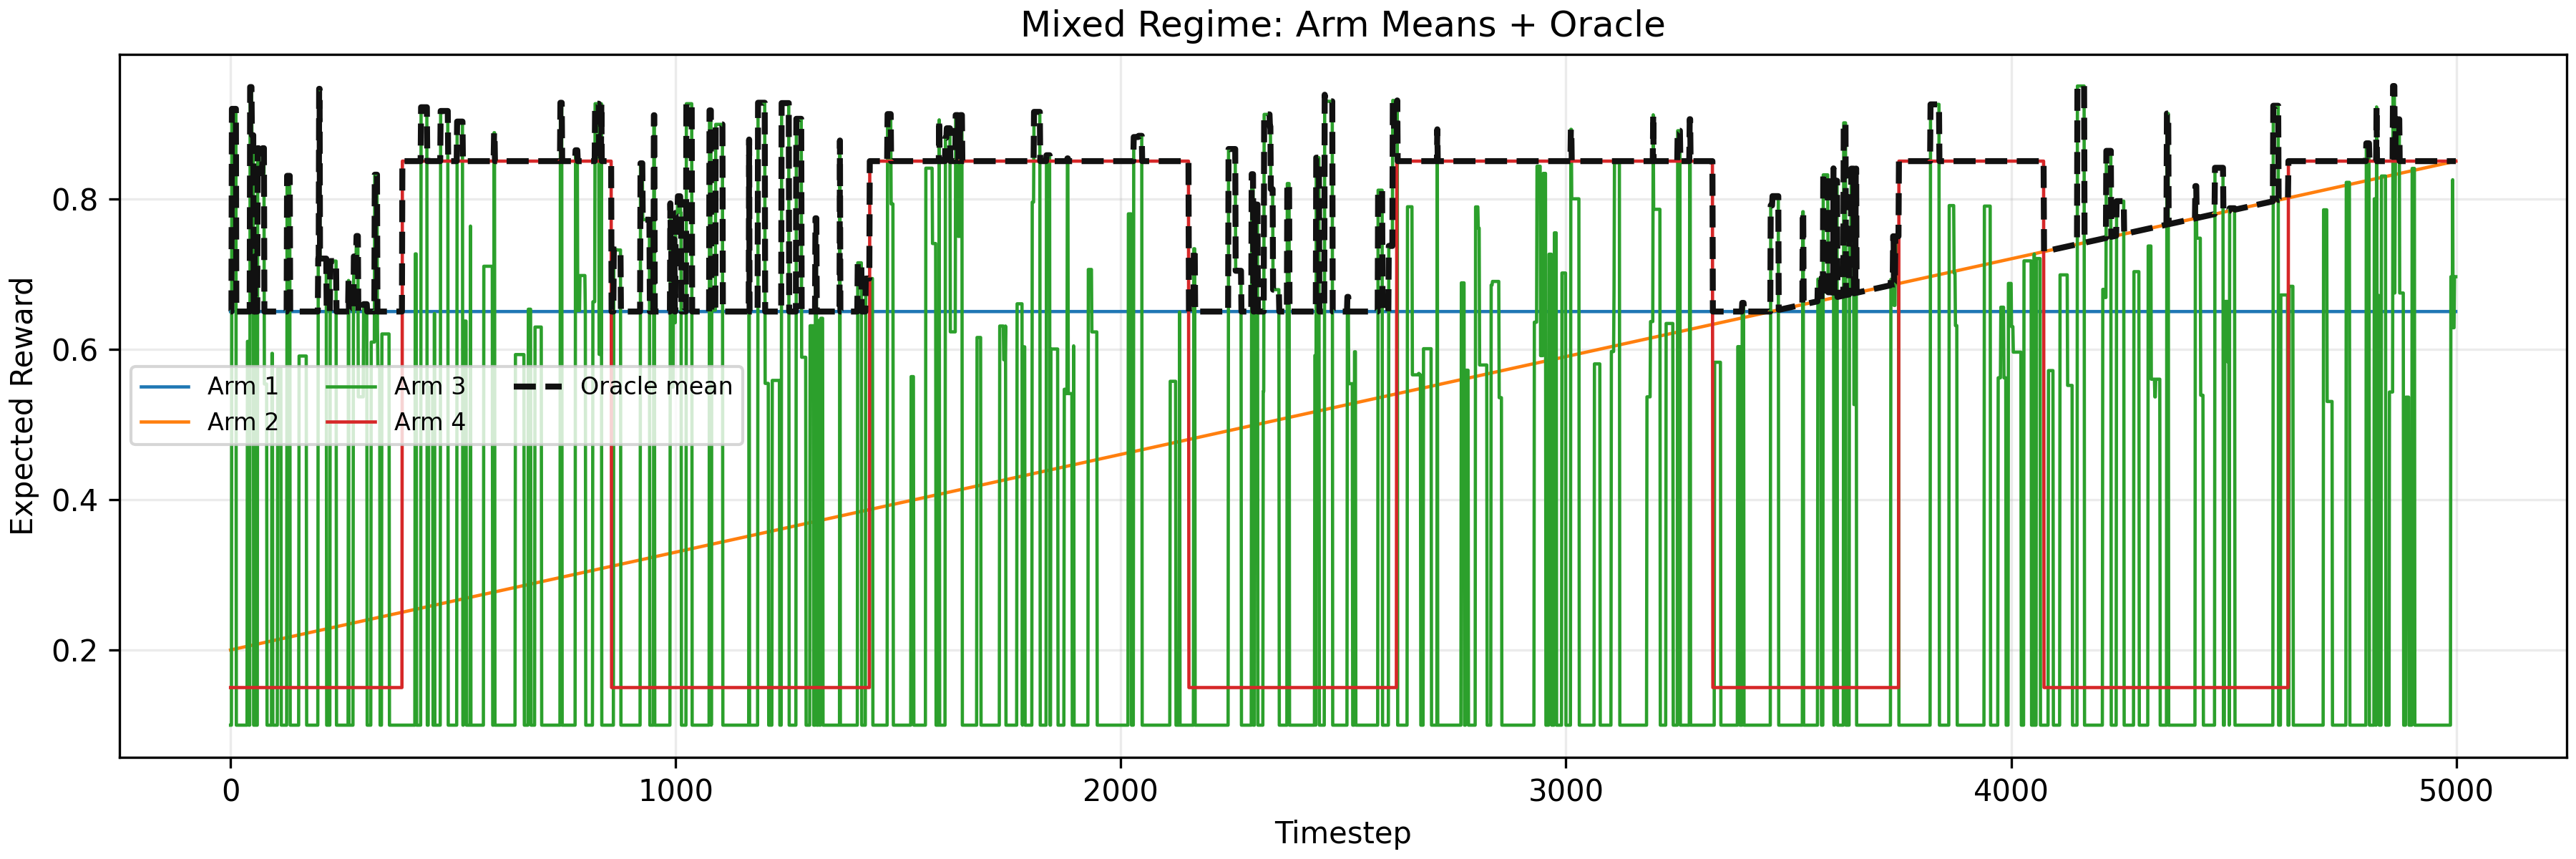
\includegraphics[width=\linewidth]{environment_oracle/environment_oracle_mixed.png}
\end{minipage}

\vspace{2mm}
\begin{minipage}[t]{0.49\textwidth}
\centering
\textbf{random\_breakpoints}\par\vspace{1mm}
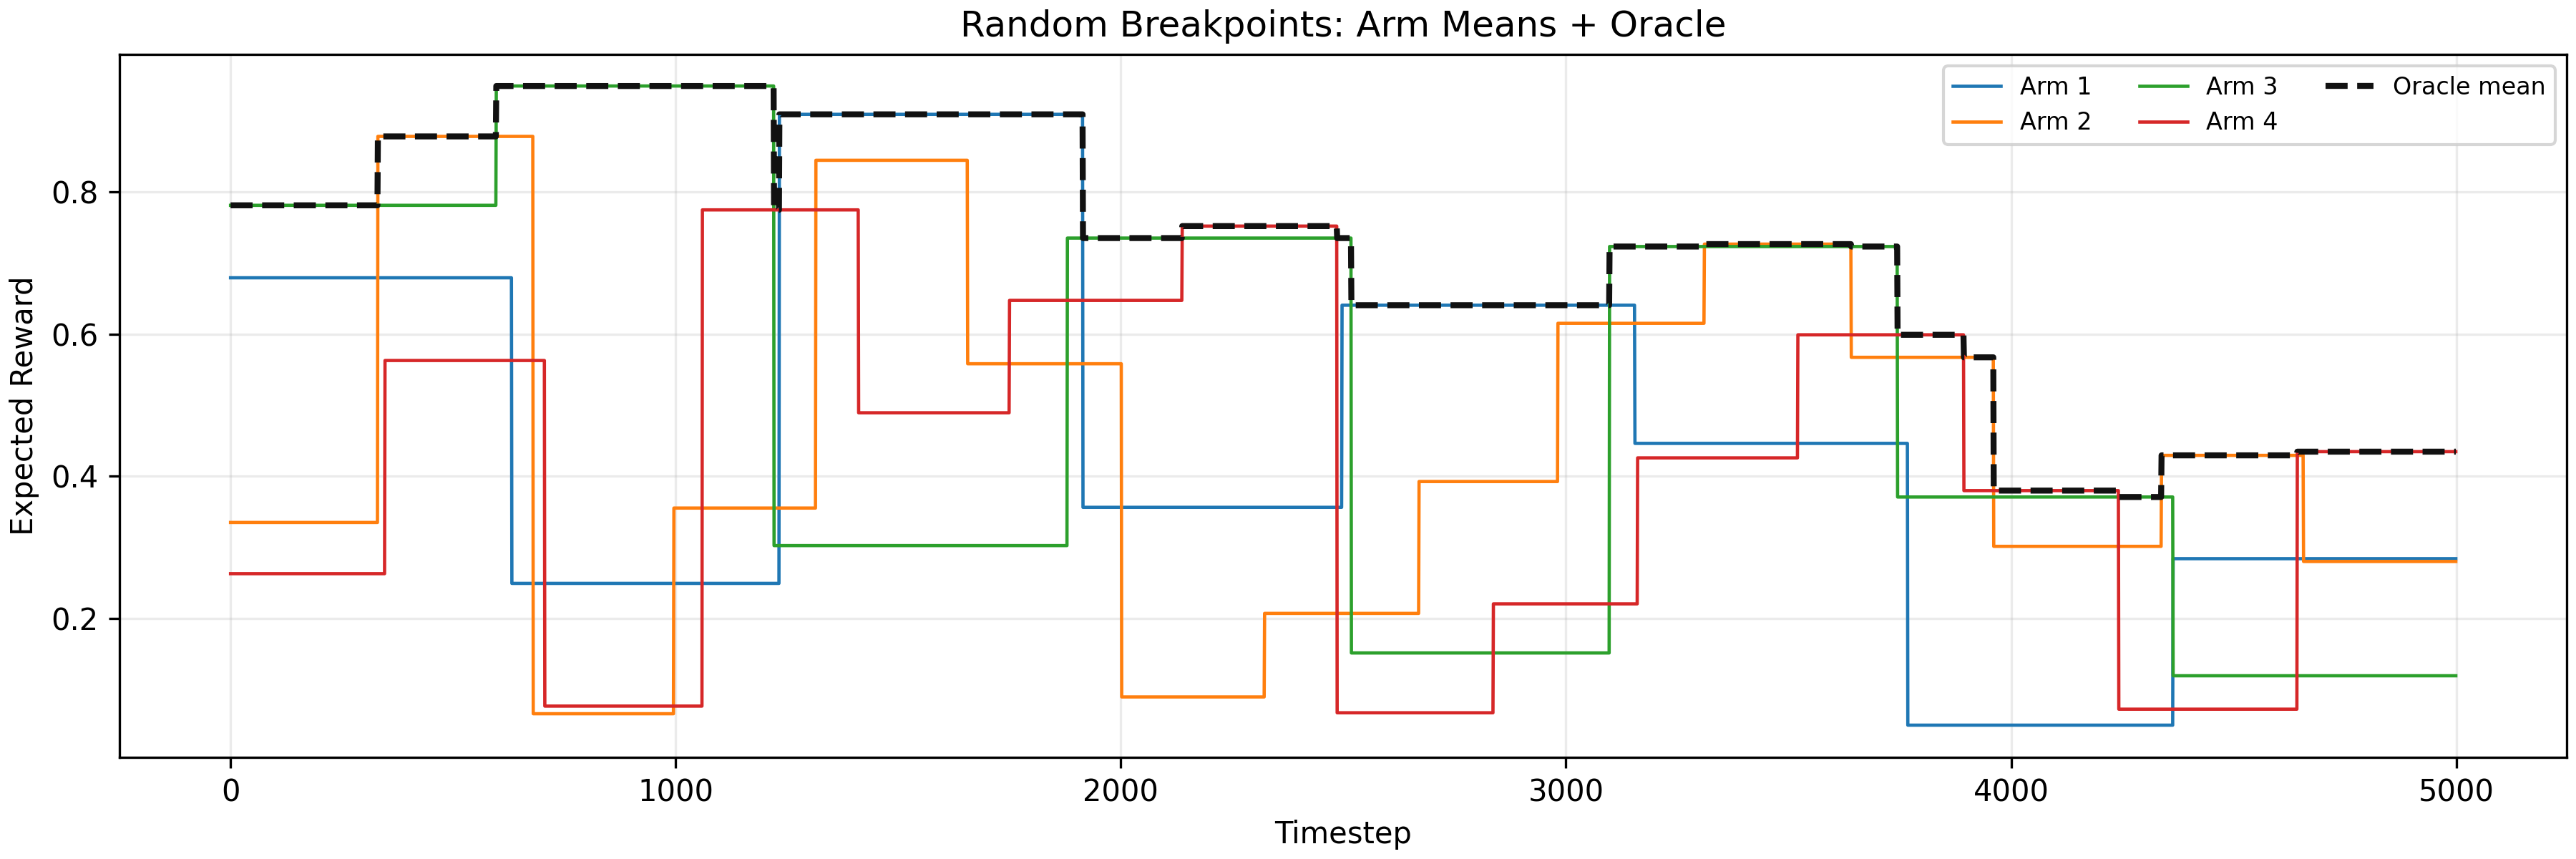
\includegraphics[width=\linewidth]{environment_oracle/environment_oracle_random_breakpoints.png}
\end{minipage}\hfill
\begin{minipage}[t]{0.49\textwidth}
\centering
\textbf{random\_drift}\par\vspace{1mm}
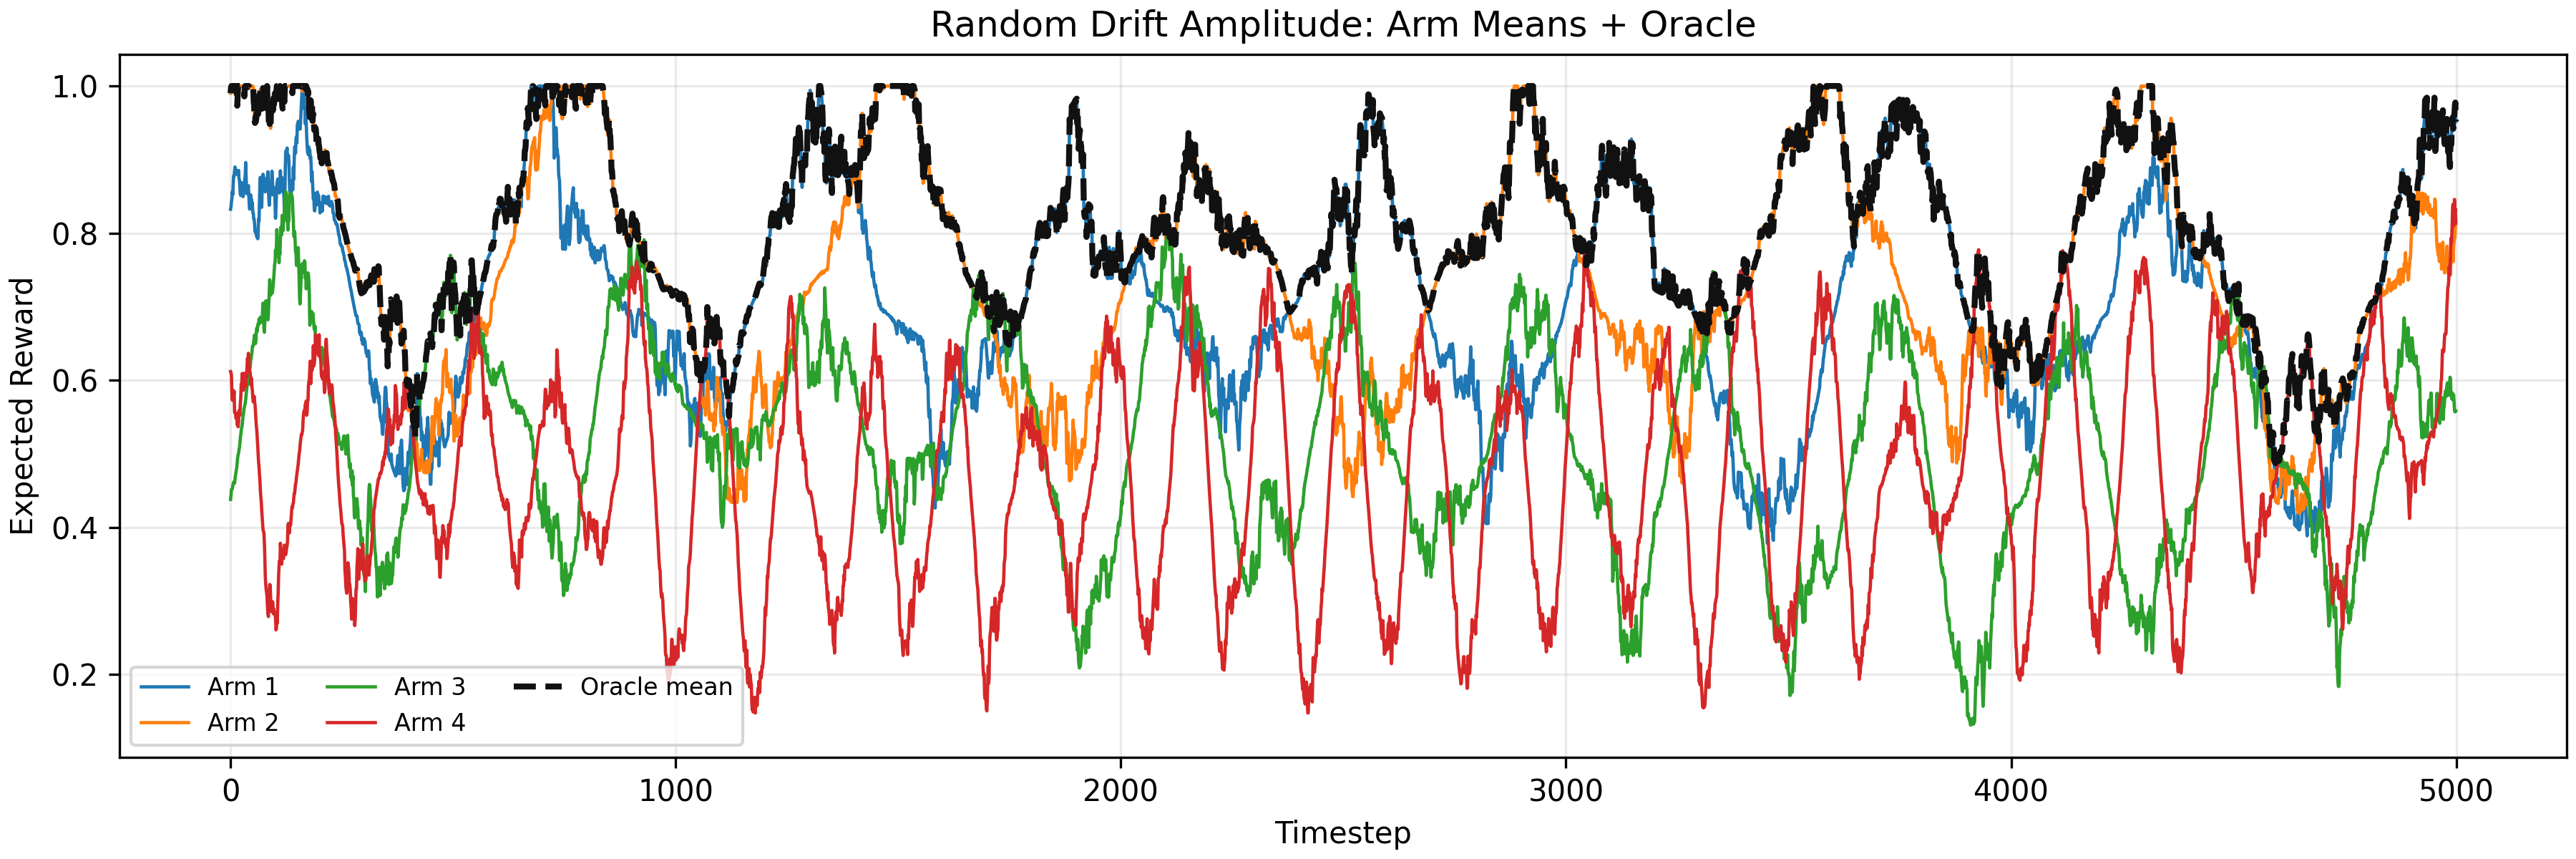
\includegraphics[width=\linewidth]{environment_oracle/environment_oracle_random_drift.png}
\end{minipage}

\vspace{2mm}
\begin{minipage}[t]{0.49\textwidth}
\centering
\textbf{global\_switching}\par\vspace{1mm}
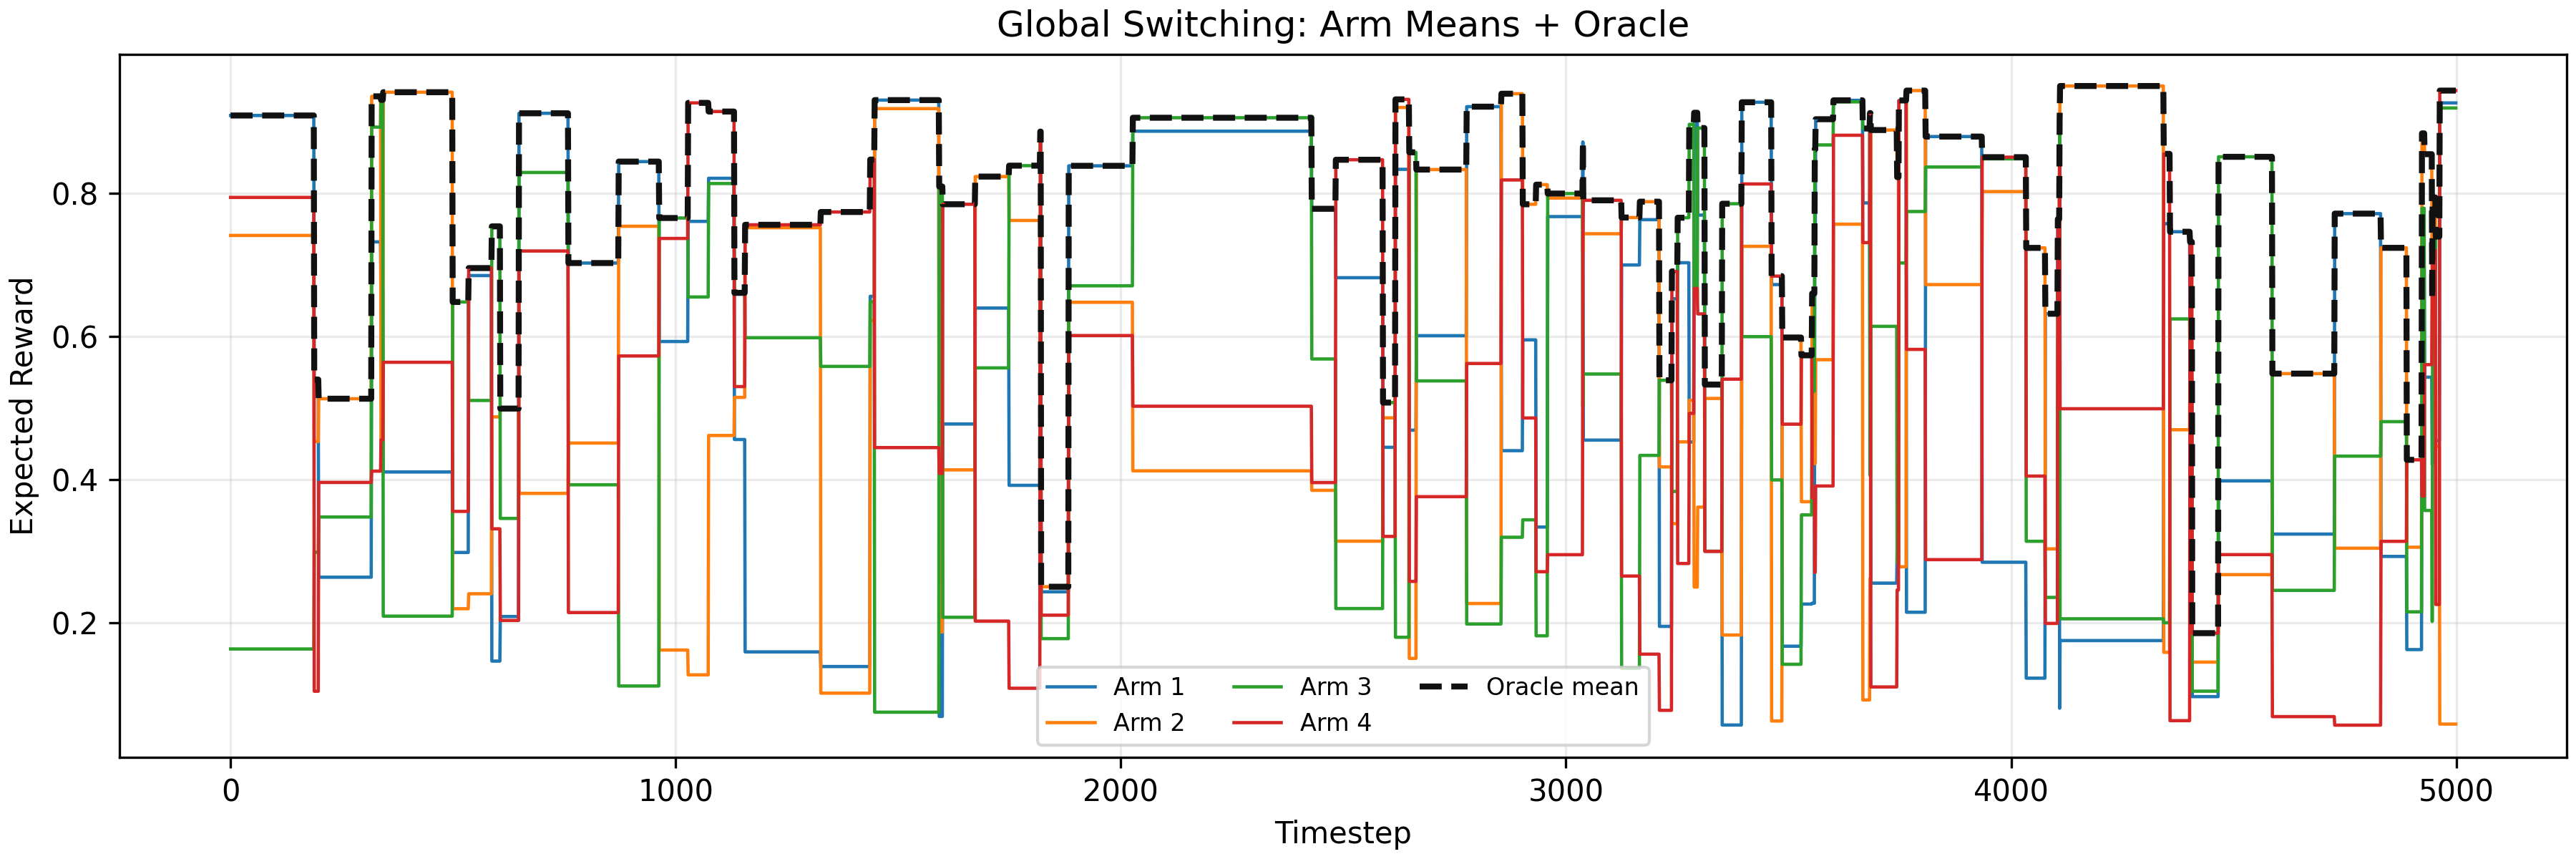
\includegraphics[width=\linewidth]{environment_oracle/environment_oracle_global_switching.png}
\end{minipage}\hfill
\begin{minipage}[t]{0.49\textwidth}
\centering
\textbf{per\_arm\_switching}\par\vspace{1mm}
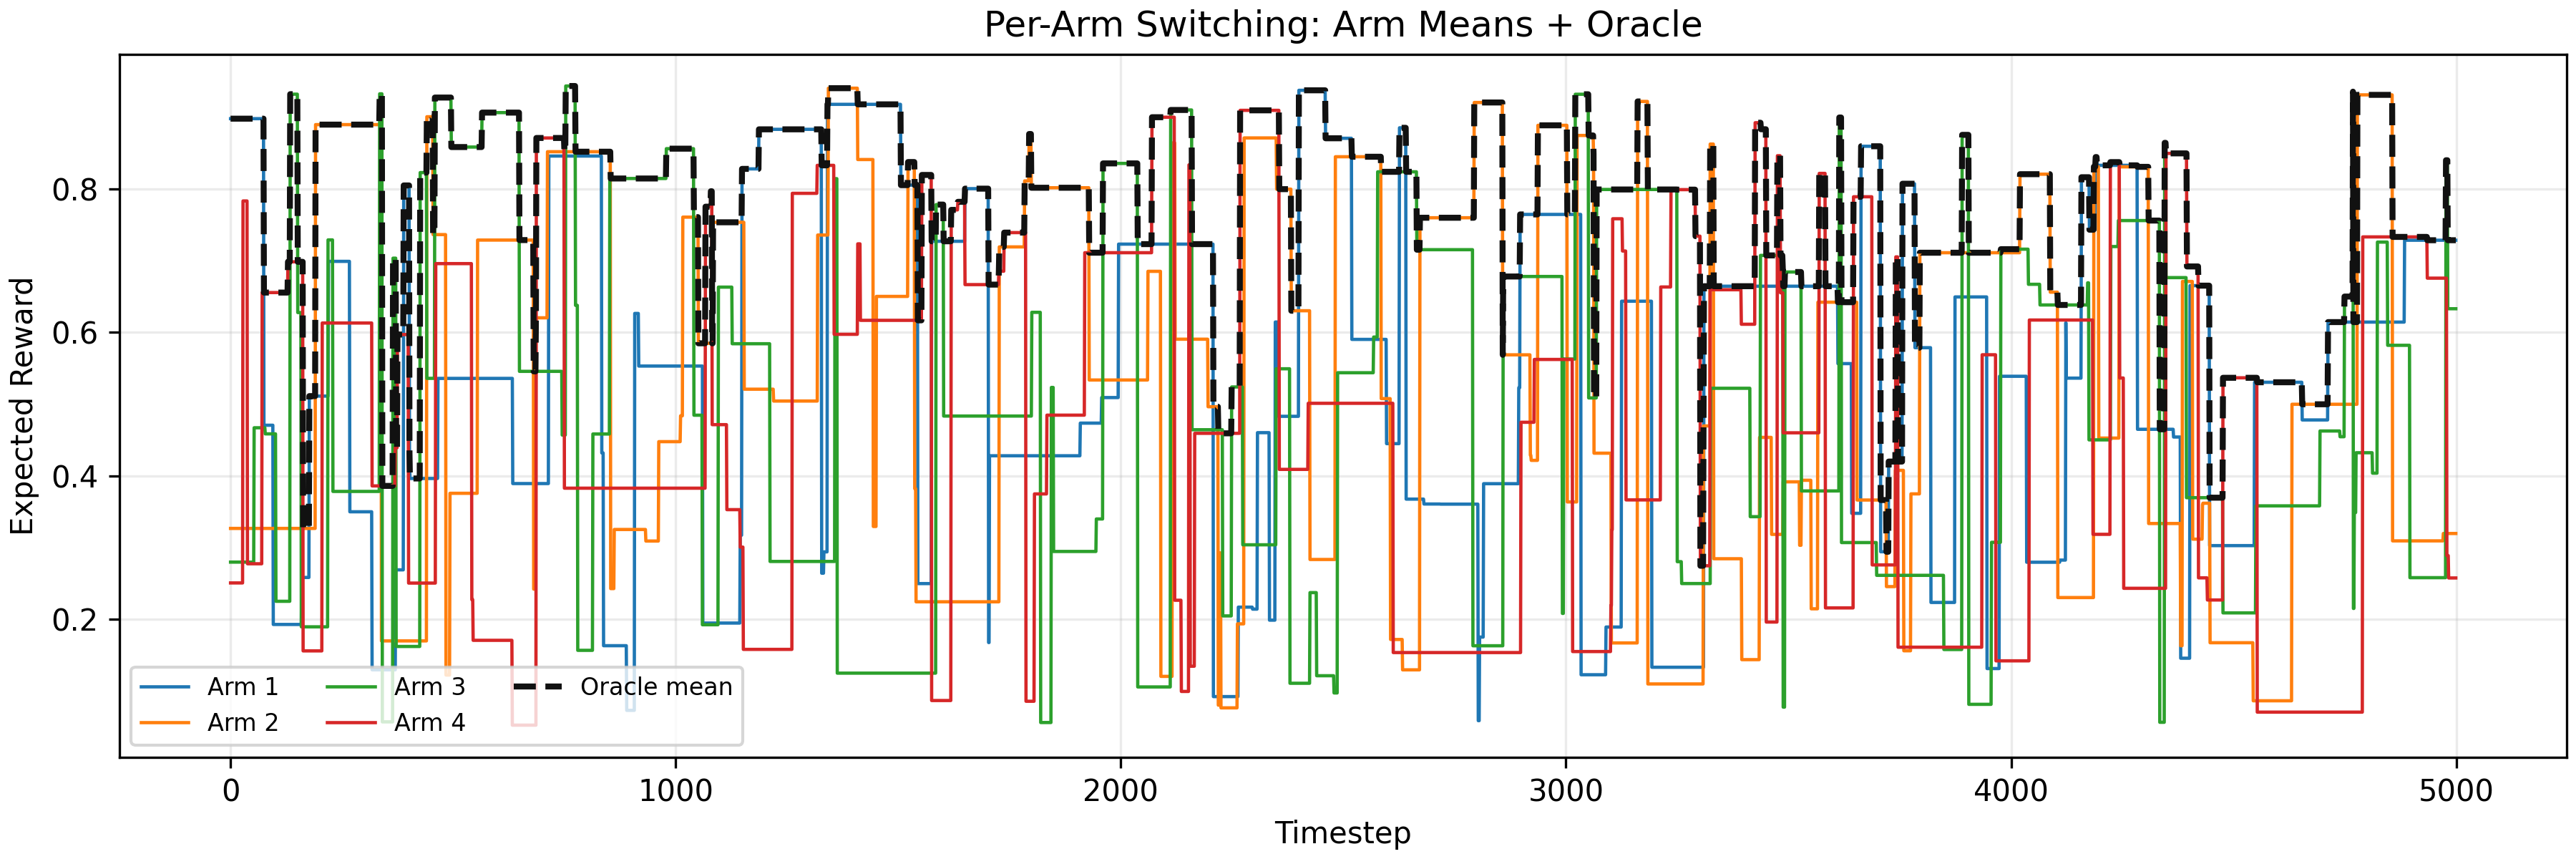
\includegraphics[width=\linewidth]{environment_oracle/environment_oracle_per_arm_switching.png}
\end{minipage}
\caption{Dynamic-oracle visualizations for all eight benchmark environments. In each subplot, the true arm means over time and the oracle mean induced by $k_t^\star=\arg\max_k \mu_{k,t}$ is shown for various environments.}
\label{fig:env_oracle_gallery}
\end{figure}

\FloatBarrier

\subsection{Tuned Performance Protocol}
By \emph{tuned performance}, we mean that each algorithm is tuned separately for each environment using the same target metric: final normalized regret. For every policy-environment pair, we select the hyperparameters that minimize \texttt{tuning\_final\_normalized\_regret}, then report \texttt{eval\_final\_normalized\_regret} under the selected setting.

The tuned hyperparameters are the primary adaptation controls for each method: none for TS; discount factor for dTS/dOTS (faster adaptation at lower values); $(\lambda, C)$ for Dynamic TS, where $C$ is the played arm's posterior-mass threshold and the effective discount is $\lambda=\frac{C}{C+1}$ (equivalently, $C=\frac{\lambda}{1-\lambda}$ in our tuned sweep); $(\gamma,\Delta)$ for REXP3, where $\gamma$ is exploration rate and $\Delta$ is restart window length; window length $\tau$ for Beta-SWTS; and VG-dTS controls $(\gamma_{\min},\gamma_{\mathrm{def}},n_0,\lambda_{\mathrm{vol}})$ plus surprise-mapping settings, where $n_0$ is gate strength and $s_t\!\rightarrow\!\nu_{k,t}\!\rightarrow\!\gamma^{\mathrm{vol}}_{k,t}$ is the surprise-to-discount path used in Algorithm~\ref{alg:vgdts}.

The family-specific search grids have unequal sizes: VG-dTS has 64 candidates; dTS, dOTS, and Dynamic TS have 7 each; TS has 1; REXP3 has 15; and Beta-SWTS has 5. Thus equal rollouts per candidate do not imply equal tuning budgets, and the tuned comparison does not isolate algorithmic quality from search effort.
For horizon $T=5000$, the baseline grids are:
dTS/dOTS and Dynamic TS: $\lambda\in\{0.30,0.45,0.60,0.75,0.85,0.92,0.97\}$, with Dynamic TS mapped to $C=\lambda/(1-\lambda)$.
REXP3: $\gamma\in\{0.05,0.10,0.20,0.30,0.40\}$ and $\Delta\in\{125,250,500\}$.
Beta-SWTS: $\tau\in\{50,100,200,500,1000\}$.
The VG-dTS grid varies six controls:
$\gamma_{\mathrm{def}}\in\{0.45,0.85\}$,
$\gamma_{\min}\in\{0.12,0.70\}$,
$\lambda_{\mathrm{vol}}\in\{0.88,0.97\}$,
$n_0\in\{0,25\}$,
$\nu_{\mathrm{high}}\in\{2.6,3.5\}$, and
one-sided surprise flag $b\in\{0,1\}$, where $b=1$ uses downside-only surprise $e_t=\max\{\bar{\mu}_{A_t,t}-x_t,0\}$ and $b=0$ uses two-sided surprise $e_t=|x_t-\bar{\mu}_{A_t,t}|$.
All VG-dTS candidates use optimistic scoring, the inverse-linear map, $\gamma_{\max}=0.995$, $\nu_{\mathrm{low}}=0$, $c=8$, $\epsilon=10^{-12}$, $(m_k,v_k)=(0,0)$ initially, and a $\mathrm{Beta}(1,1)$ prior. The same prior is used for the other Beta-based policies. Tuned results evaluate the setting selected from each specified grid on that environment realization; they are not estimates of an unconstrained best-case capability. The fixed protocol instead evaluates one archived setting per method across the suite.

\subsection{Results on Canonical Benchmarks}
Figure~\ref{fig:original_paper_envs_tuned} summarizes tuned results on \texttt{slow}, \texttt{fast}, and \texttt{abrupt}.
VG-dTS attains strong performance in all three regimes:
0.056 (slow), 0.211 (fast), and 0.102 (abrupt) final normalized regret.
Relative to dTS, this corresponds to improvements of 14.3\%, 12.0\%, and 17.0\%, respectively.
In abrupt dynamics, VG-dTS is best overall among all tested methods.
In fast periodic drift, VG-dTS and dOTS have similar point estimates, while both have lower reported regret than TS and REXP3. No statistical-equivalence claim is made.
These observations are consistent with a benefit from adaptive forgetting in abrupt dynamics, but this comparison does not isolate that mechanism from optimistic scoring or other configuration choices.

\begin{figure}[!htbp]
\centering
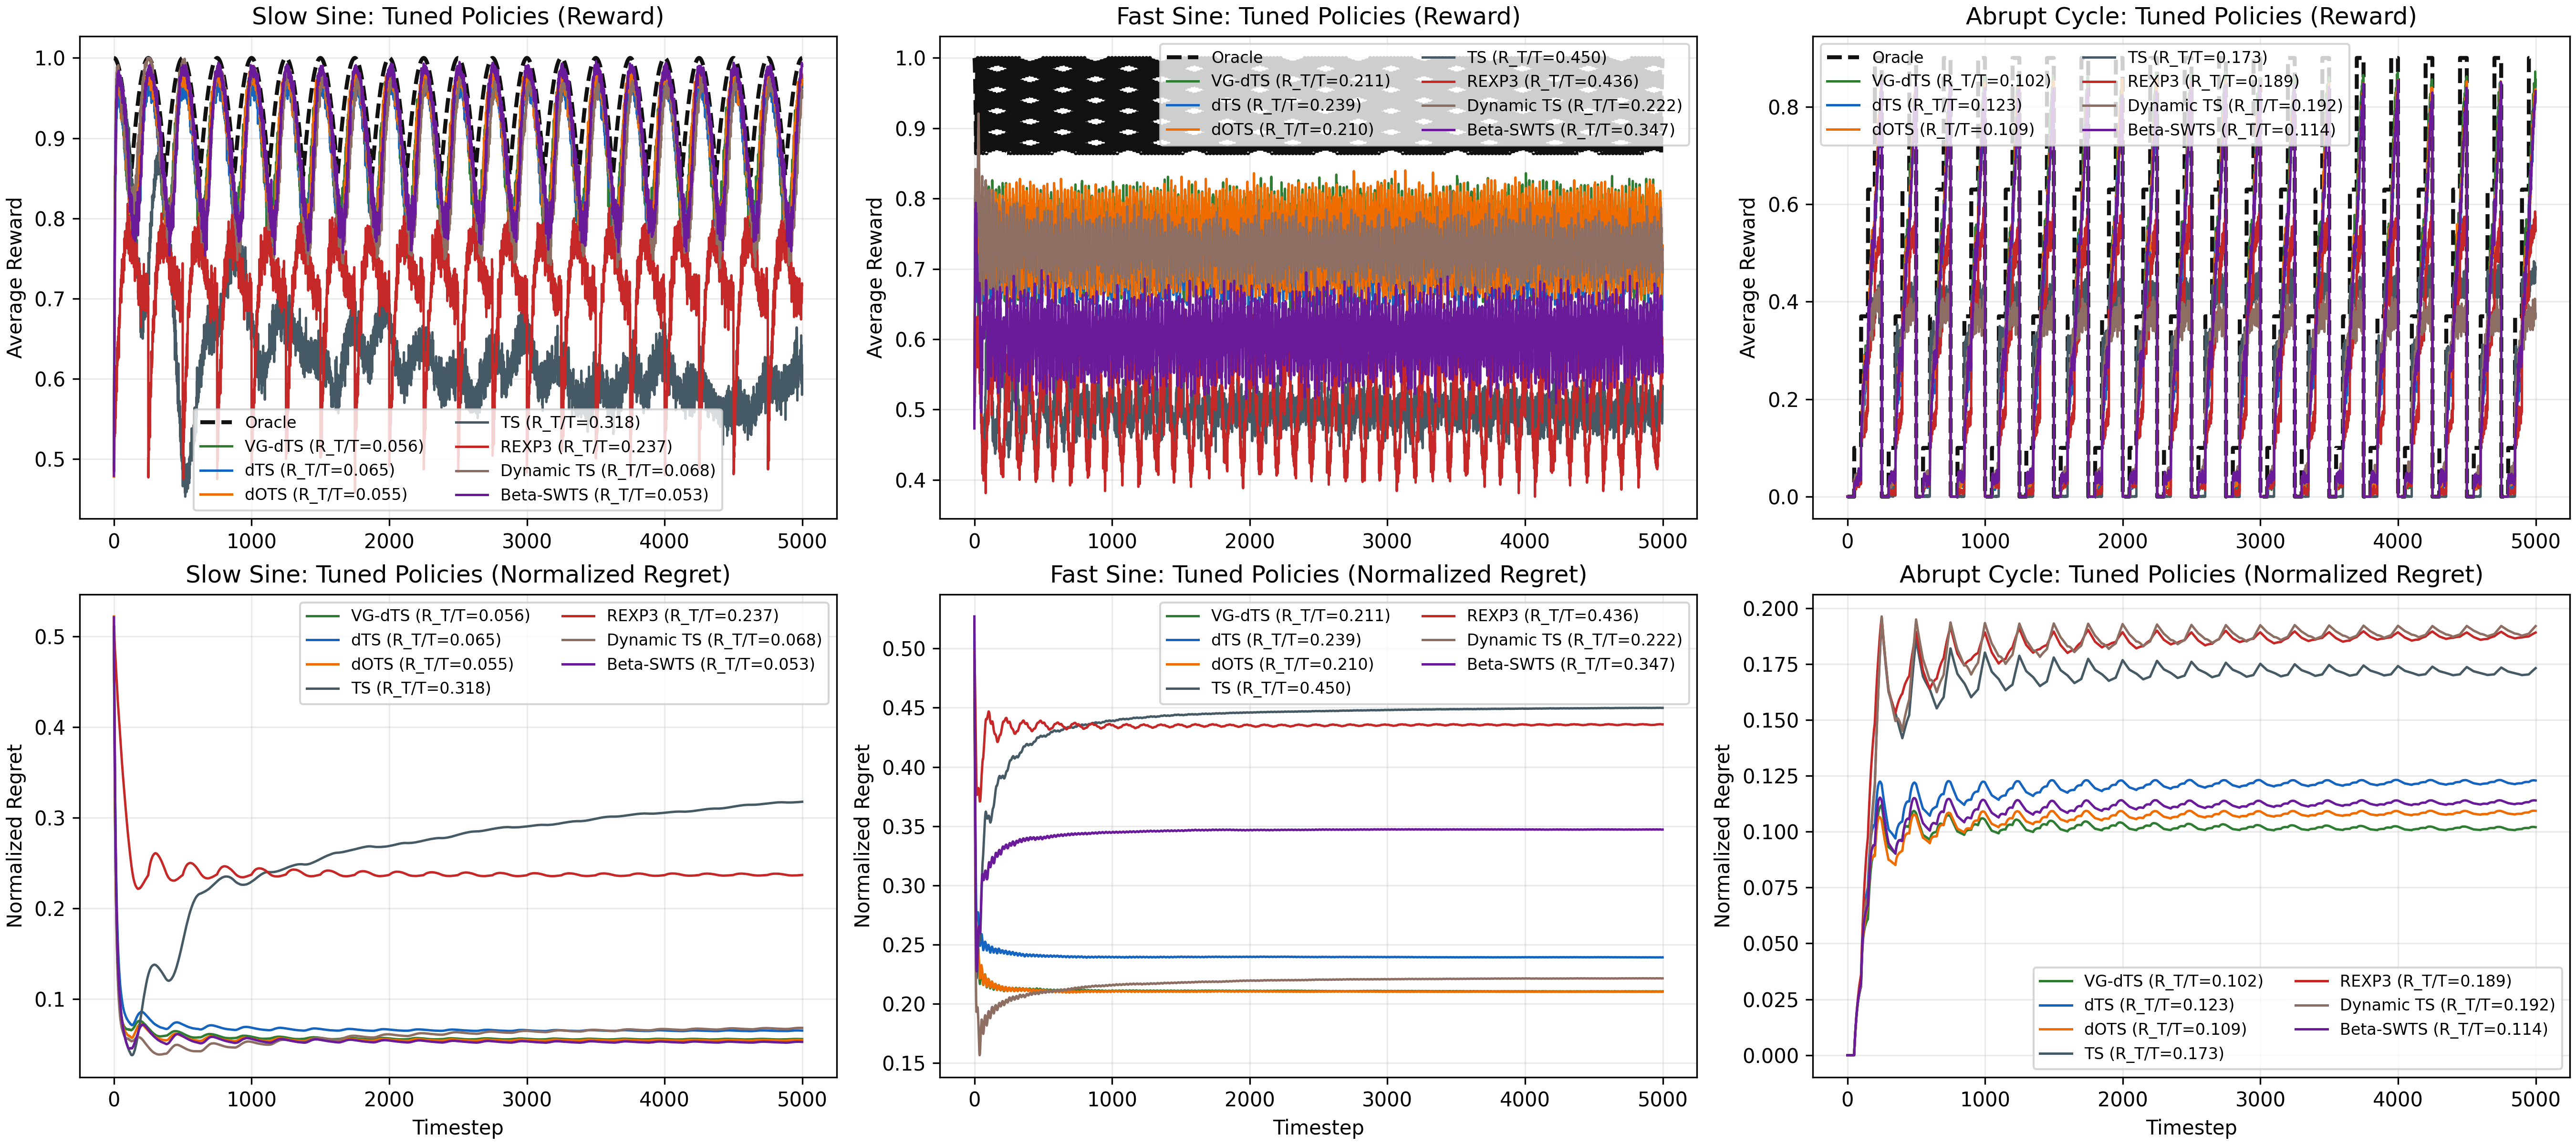
\includegraphics[width=0.98\textwidth]{original_paper_envs_tuned.png}
\caption{Tuned performance on the three canonical non-stationary environments. VG-dTS tracks top methods across all regimes and leads in abrupt changes.}
\label{fig:original_paper_envs_tuned}
\end{figure}

\FloatBarrier

\subsection{Results Across Eight Environments}
Figure~\ref{fig:optimized_heatmap} reports tuned performance across all eight environments.
VG-dTS achieves the best \emph{average} regret over the suite (0.1047), improving over dTS (0.1200), dOTS (0.1067), Dynamic TS (0.1120), and Beta-SWTS (0.1219).
The heatmap also clarifies regime specialization:
Dynamic TS is strongest in highly random switching/drift settings (\texttt{random\_breakpoints}, \texttt{random\_drift}, \texttt{global\_switching}, \texttt{per\_arm\_switching}),
while VG-dTS is strongest on \texttt{abrupt} and near-best on \texttt{slow}, \texttt{fast}, and \texttt{mixed}.
These are descriptive rankings on the evaluated realizations; the experiment does not identify the mechanism responsible for each difference.
Table~\ref{tab:tuned_params_matrix} summarizes the selected controls. All eight selected VG-dTS settings use $\nu_{\mathrm{high}}=3.5$; only \texttt{fast} selects $n_0=25$, while the other seven select $n_0=0$. Supplied defaults of $0.45$ in \texttt{mixed} and \texttt{random\_drift} are clipped to $\gamma_{\min}=0.70$ before mixing. Full-precision parameter dictionaries are archived in the repository.

\begin{figure}[H]
\centering
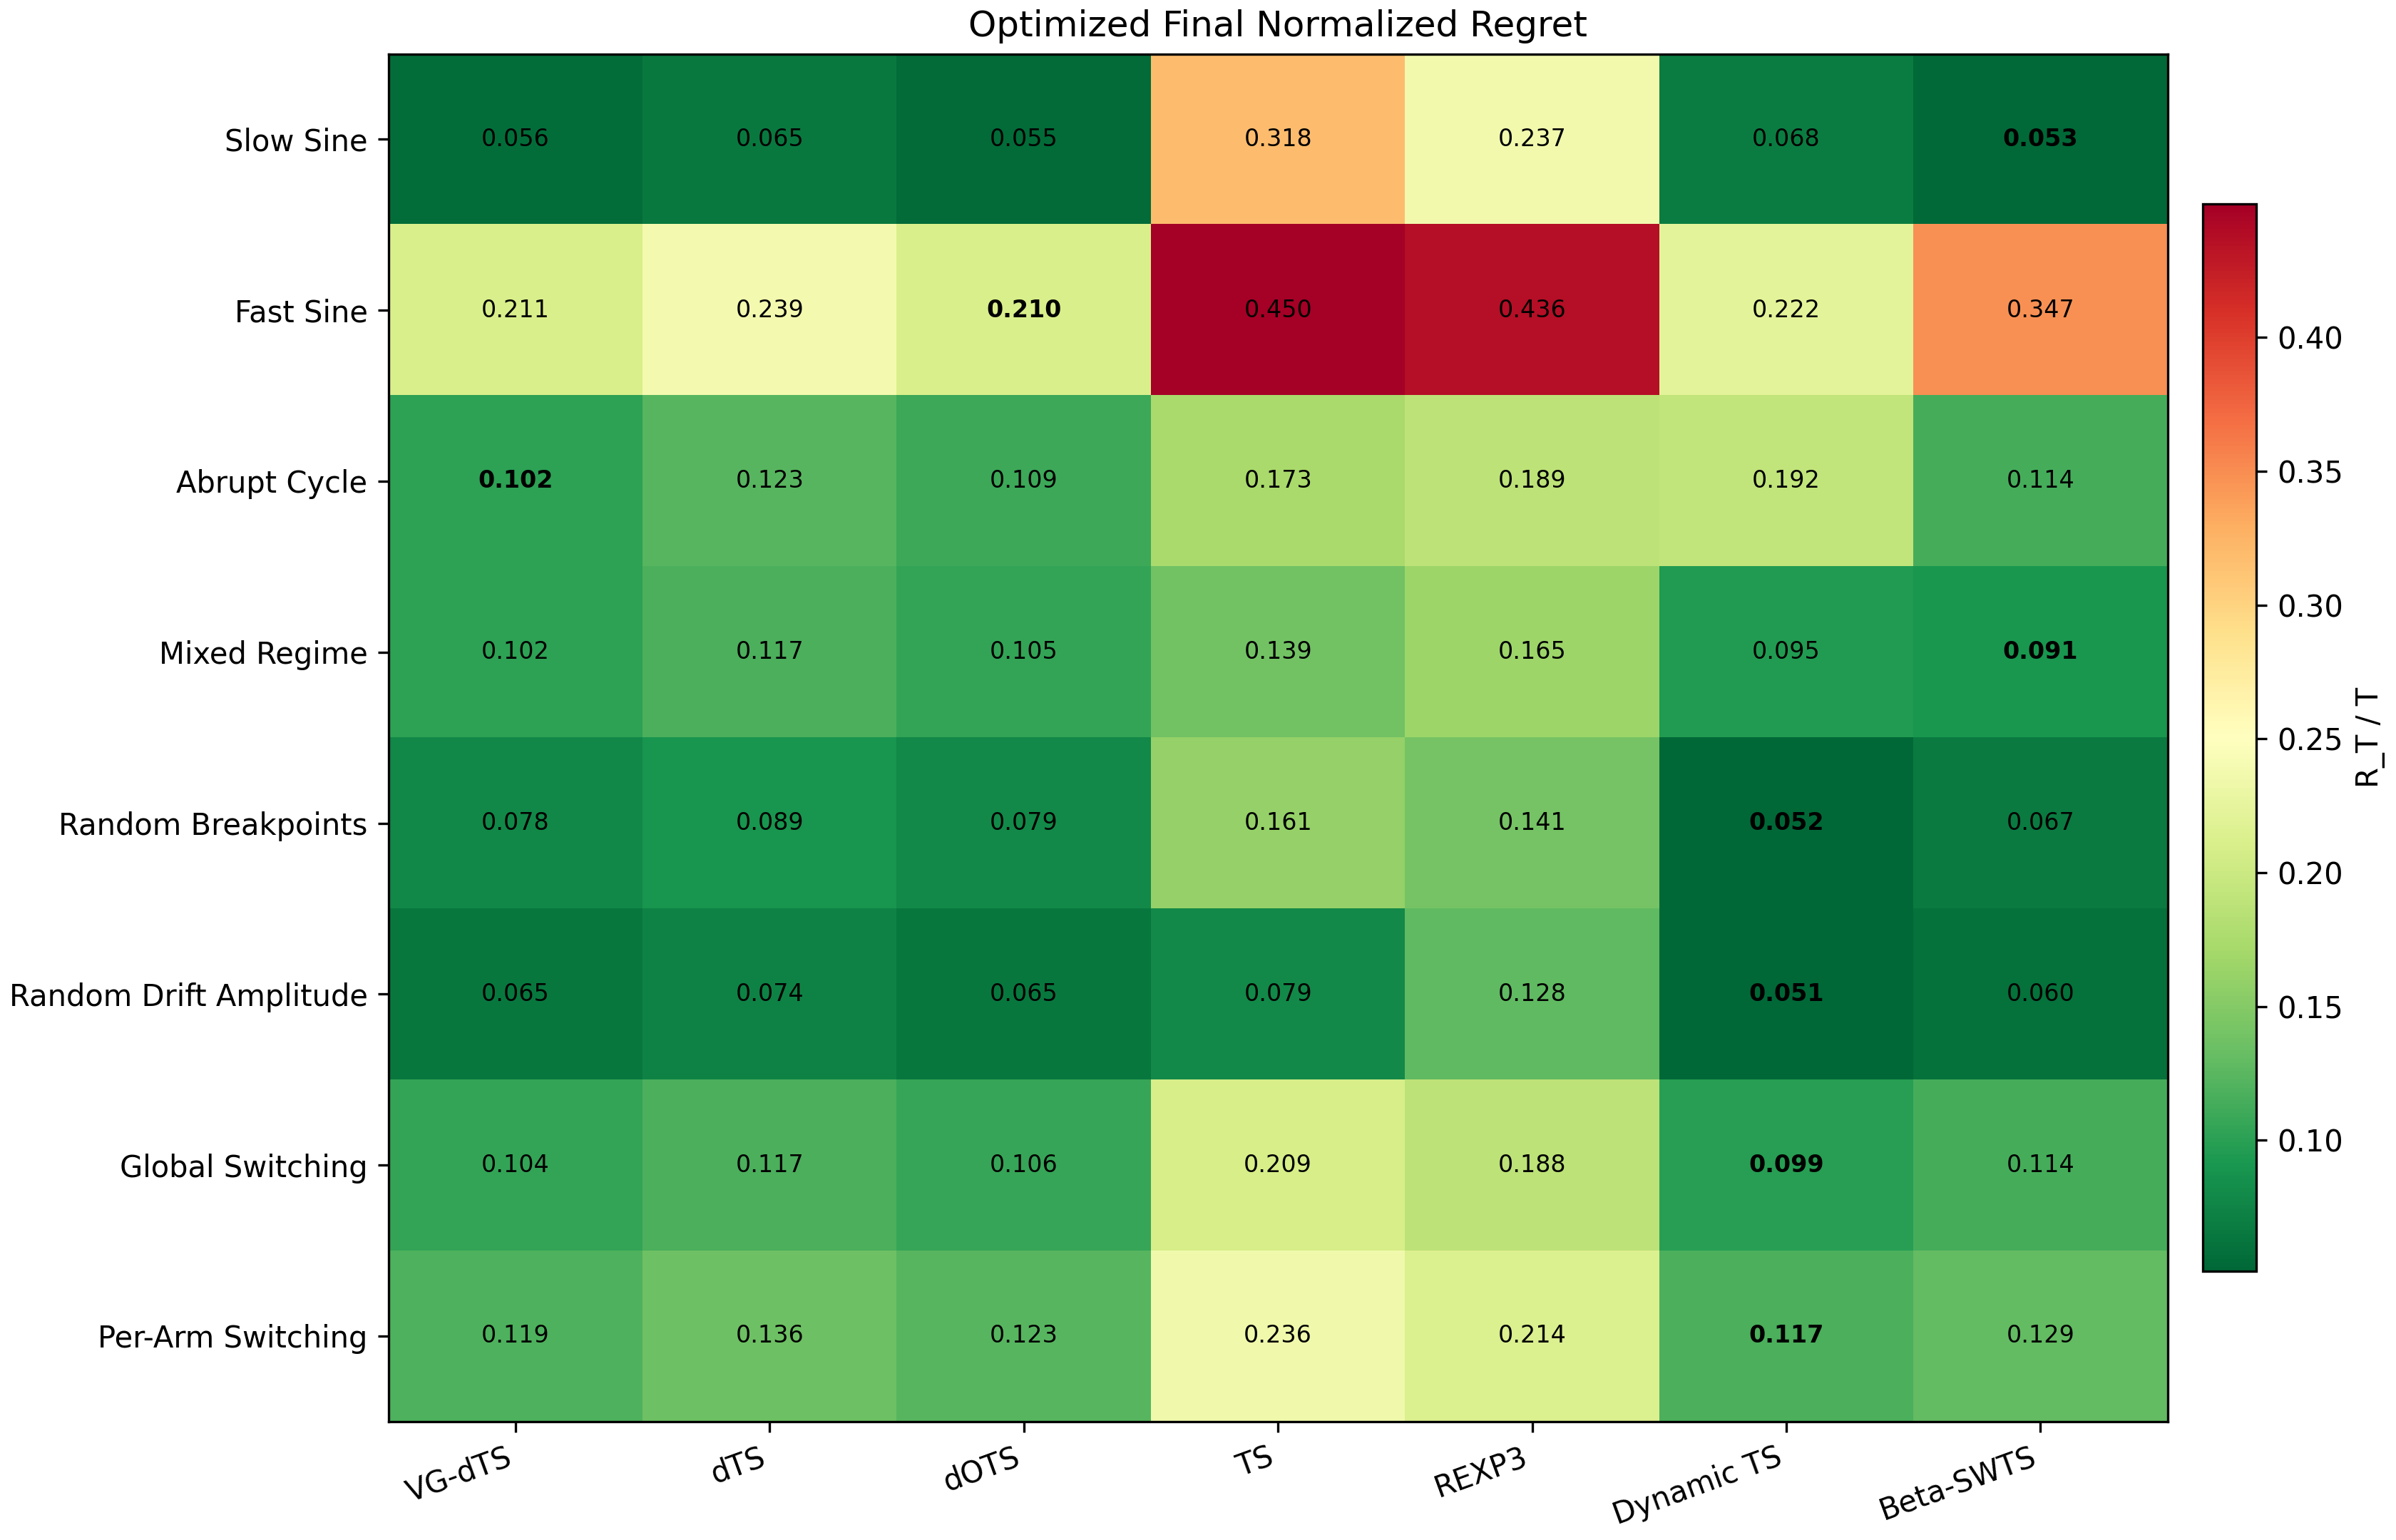
\includegraphics[width=0.98\textwidth]{optimized_heatmap_8env_7policies.png}
\caption{Tuned final normalized regret across eight environments and seven algorithms (lower is better).}
\label{fig:optimized_heatmap}
\end{figure}

\begin{table}[H]
\centering
\scriptsize
\setlength{\tabcolsep}{3pt}
\renewcommand{\arraystretch}{1.15}
\resizebox{\textwidth}{!}{
\begin{tabular}{lccccccc}
\toprule
Environment & VG-dTS & dTS & dOTS & TS & REXP3 & Dynamic TS & Beta-SWTS \\
\midrule
\texttt{slow} & (0.88,0.70,0.85,0,0) & 0.97 & 0.97 & -- & (0.2,250) & (0.75,3.0) & 100 \\
\texttt{fast} & (0.88,0.12,0.85,25,0) & 0.85 & 0.85 & -- & (0.4,125) & (0.60,1.5) & 50 \\
\texttt{abrupt} & (0.97,0.70,0.85,0,1) & 0.97 & 0.97 & -- & (0.3,500) & (0.97,32.33) & 50 \\
\texttt{mixed} & (0.88,0.70,0.45,0,0) & 0.97 & 0.97 & -- & (0.2,500) & (0.85,5.67) & 100 \\
\texttt{random\_breakpoints} & (0.88,0.70,0.85,0,0) & 0.97 & 0.97 & -- & (0.2,500) & (0.92,11.50) & 100 \\
\texttt{random\_drift} & (0.88,0.70,0.45,0,0) & 0.97 & 0.97 & -- & (0.2,500) & (0.92,11.50) & 100 \\
\texttt{global\_switching} & (0.88,0.70,0.85,0,0) & 0.97 & 0.97 & -- & (0.2,500) & (0.75,3.0) & 50 \\
\texttt{per\_arm\_switching} & (0.88,0.70,0.85,0,0) & 0.97 & 0.97 & -- & (0.4,125) & (0.75,3.0) & 50 \\
\bottomrule
\end{tabular}
}
\caption{Selected tuned controls (env rows, algorithm columns); Dynamic TS thresholds are rounded. Common VG-dTS constants are specified in the text, including $\nu_{\mathrm{high}}=3.5$ and optimistic scoring. The $\gamma_{\mathrm{def}}$ tuple entry reports the supplied value before clipping. Notation: VG-dTS cells use $(\lambda_{\mathrm{vol}},\gamma_{\min},\gamma_{\mathrm{def}},n_0,b)$ with fixed $\gamma_{\max}=0.995$, where $b\in\{0,1\}$ selects surprise mode ($b=1$: downside-only, $b=0$: two-sided); dTS/dOTS cells show $\gamma$; REXP3 cells show $(\gamma,\Delta)$; Dynamic TS cells show $(\lambda,C)$; Beta-SWTS cells show $\tau$; TS has no tuned hyperparameter.}
\label{tab:tuned_params_matrix}
\end{table}

\FloatBarrier

\subsection{Robustness and Noise Stress Test}
Figure~\ref{fig:fixed_heatmap} removes per-environment retuning by using fixed parameters across all environments.
Under this stricter protocol, VG-dTS has the best average regret (0.1351), a 33.5\% reduction versus dTS and 24.2\% versus dOTS, and ties for most per-environment wins.
This establishes a lower average for the particular fixed configurations evaluated. It does not establish insensitivity to parameter choice or a causal benefit from the reliability gate.
The fixed controls are listed in Table~\ref{tab:fixed_params_matrix}; full-precision settings are archived in the repository.

The archived settings in Figure~\ref{fig:fixed_heatmap} and Table~\ref{tab:fixed_params_matrix} are held constant across environments. The archive does not document an independent procedure for selecting these defaults, so this protocol should not be interpreted as held-out environment selection.
For VG-dTS, we use the benchmark default tuple $(\lambda_{\mathrm{vol}},\gamma_{\min},\gamma_{\mathrm{def}},n_0,b)=(0.88,0.12,0.45,0,0)$ with $\gamma_{\max}=0.995$ and $\nu_{\mathrm{high}}=2.6$. The other common VG-dTS constants match those in the tuned protocol. With $n_0=0$, the gate is fully open whenever effective evidence is positive; these fixed results therefore do not demonstrate a benefit from gradual reliability gating.
For dTS/dOTS, $\gamma=0.75$ is a mid-range memory setting from the tuned grid.
For REXP3, $(\gamma,\Delta)=(0.1136,250)$ sets the exploration mixture weight to $0.1136$ and restarts the weights every 250 rounds.
For Dynamic TS, $C=250$ (equivalently $\lambda=\frac{C}{C+1}\approx 0.996$) delays discounting until the played arm exceeds the posterior-mass threshold and then uses mild discounting.
For Beta-SWTS, $\tau=200$ retains observations from the most recent 200 rounds ($4\%$ of the horizon at $T=5000$).

Figure~\ref{fig:pure_random_signal} shows a tuned negative control (\texttt{pure\_random\_signal}) whose arm means are independently drawn from $\mathrm{Uniform}(0.05,0.95)$ at every round. One realization is held fixed across rollouts, with the same tuning grids and rollout budgets as above. The methods have close reported point estimates:
the spread between best and worst final normalized regret is only $6.13\times 10^{-4}$.
This is consistent with past rewards providing no predictive information about the next independent draw of arm means. It does not establish statistical equivalence between methods.

\begin{figure}[!htbp]
\centering
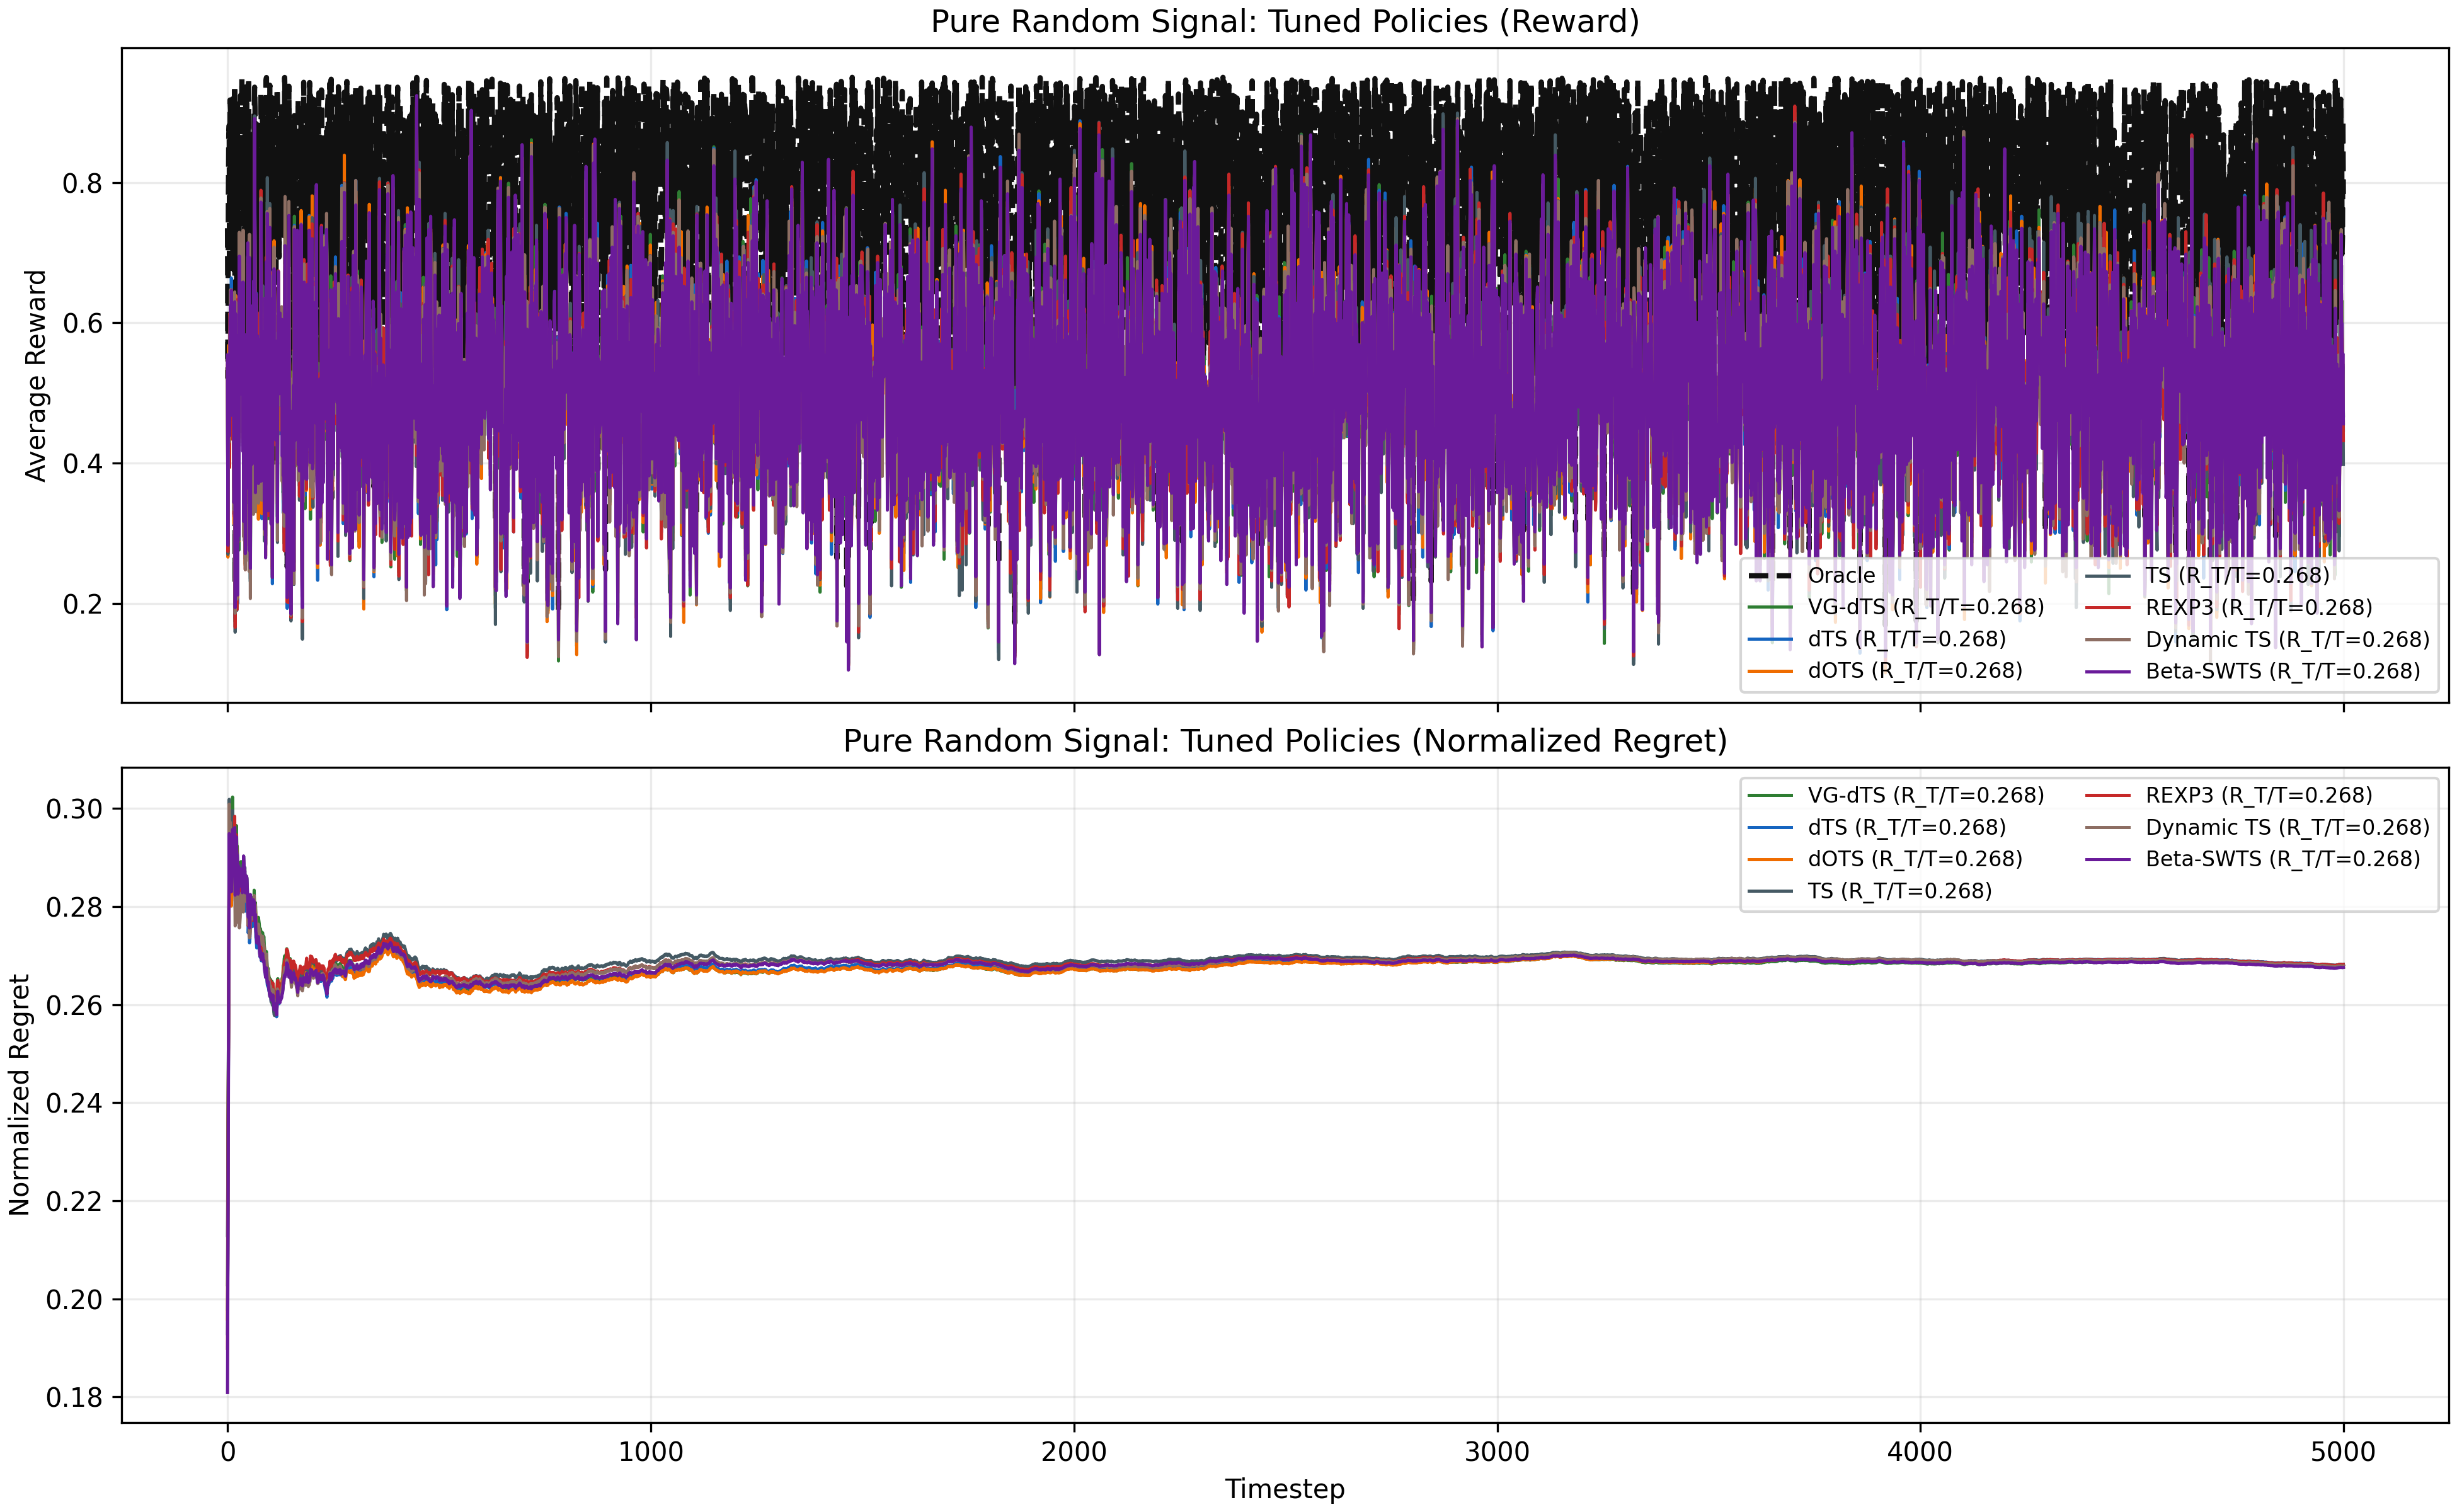
\includegraphics[width=\linewidth]{rigorous_pure_random_signal_tuned.png}
\caption{Tuned pure-random-signal control: reported final regrets differ by at most $6.13\times10^{-4}$ on this realization. No confidence intervals or equivalence test are reported.}
\label{fig:pure_random_signal}
\end{figure}

\FloatBarrier
\clearpage

\begin{figure}[H]
\centering
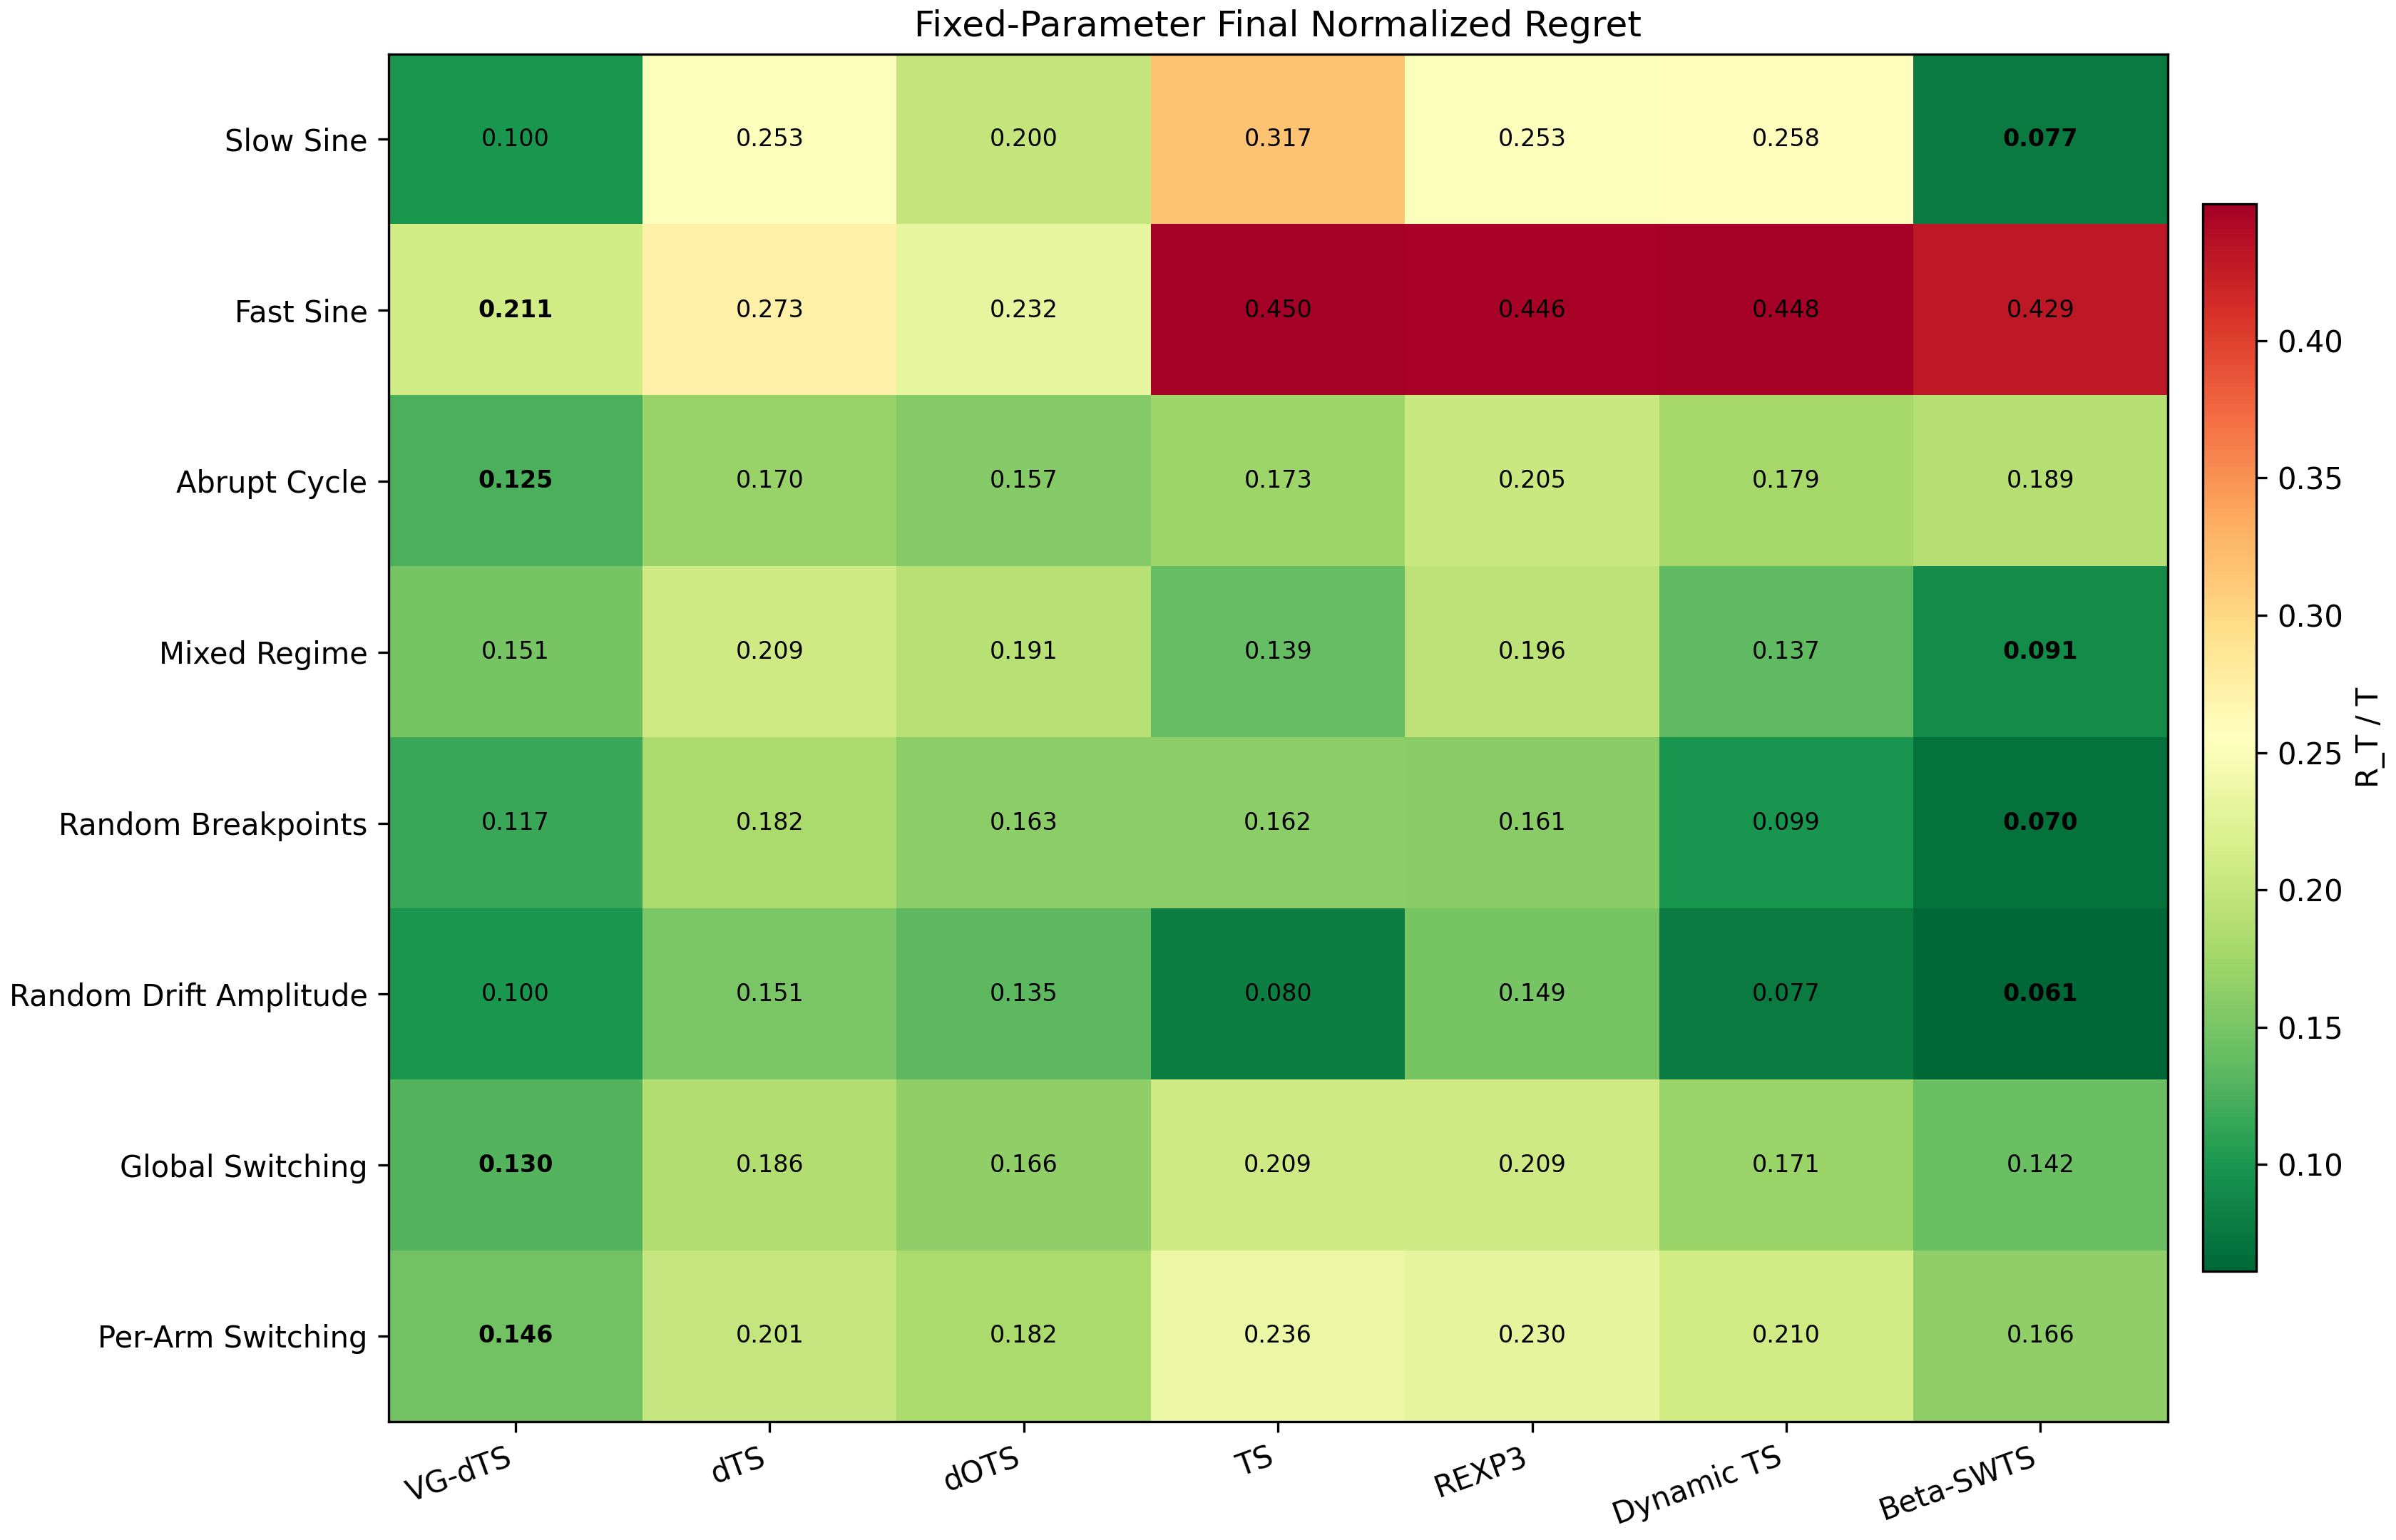
\includegraphics[width=0.98\textwidth]{fixed_params_heatmap_8env_7policies.png}
\caption{Fixed-parameter robustness across the same eight environments (lower is better). VG-dTS remains consistently competitive without per-environment tuning.}
\label{fig:fixed_heatmap}
\end{figure}

\begin{table}[H]
\centering
\scriptsize
\setlength{\tabcolsep}{3pt}
\renewcommand{\arraystretch}{1.15}
\resizebox{\textwidth}{!}{
\begin{tabular}{lccccccc}
\toprule
Environment & VG-dTS & dTS & dOTS & TS & REXP3 & Dynamic TS & Beta-SWTS \\
\midrule
\texttt{slow} & (0.88,0.12,0.45,0,0) & 0.75 & 0.75 & -- & (0.1136,250) & (0.996,250) & 200 \\
\texttt{fast} & (0.88,0.12,0.45,0,0) & 0.75 & 0.75 & -- & (0.1136,250) & (0.996,250) & 200 \\
\texttt{abrupt} & (0.88,0.12,0.45,0,0) & 0.75 & 0.75 & -- & (0.1136,250) & (0.996,250) & 200 \\
\texttt{mixed} & (0.88,0.12,0.45,0,0) & 0.75 & 0.75 & -- & (0.1136,250) & (0.996,250) & 200 \\
\texttt{random\_breakpoints} & (0.88,0.12,0.45,0,0) & 0.75 & 0.75 & -- & (0.1136,250) & (0.996,250) & 200 \\
\texttt{random\_drift} & (0.88,0.12,0.45,0,0) & 0.75 & 0.75 & -- & (0.1136,250) & (0.996,250) & 200 \\
\texttt{global\_switching} & (0.88,0.12,0.45,0,0) & 0.75 & 0.75 & -- & (0.1136,250) & (0.996,250) & 200 \\
\texttt{per\_arm\_switching} & (0.88,0.12,0.45,0,0) & 0.75 & 0.75 & -- & (0.1136,250) & (0.996,250) & 200 \\
\bottomrule
\end{tabular}
}
\caption{Fixed controls used across environments (env rows, algorithm columns); Dynamic TS discount values are rounded. VG-dTS uses the common constants stated in the text, with $\nu_{\mathrm{high}}=2.6$ and optimistic scoring. Notation: VG-dTS cells use $(\lambda_{\mathrm{vol}},\gamma_{\min},\gamma_{\mathrm{def}},n_0,b)$ with fixed $\gamma_{\max}=0.995$, where $b\in\{0,1\}$ selects surprise mode ($b=1$: downside-only, $b=0$: two-sided); dTS/dOTS cells show $\gamma$; REXP3 cells show $(\gamma,\Delta)$; Dynamic TS cells show $(\lambda,C)$ with $\lambda=C/(C+1)$; Beta-SWTS cells show $\tau$; TS has no tuned hyperparameter.}
\label{tab:fixed_params_matrix}
\end{table}

\subsection{Discussion: When VG-dTS Helps, and When It Does Not}
VG-dTS has the lowest tuned regret on \texttt{abrupt}. Under the fixed protocol it leads on \texttt{fast}, \texttt{abrupt}, \texttt{global\_switching}, and \texttt{per\_arm\_switching}; Beta-SWTS leads on the other four environments. The fixed settings and seven of eight tuned settings use $n_0=0$, so their gains cannot be attributed to a gradual reliability gate. No reported ablation isolates the effects of the gate, optimistic scoring, or the volatility map.

The main shortcoming is that VG-dTS infers non-stationarity indirectly from reward surprise.
In the tuned stochastic switching and drift settings, the implemented threshold-discounting Dynamic TS baseline has lower regret. The present results do not establish why, and this baseline does not perform explicit change detection or posterior resets.
A second limitation is delayed volatility estimation for rarely selected arms under bandit feedback, which can slow adaptation after long inactivity.
\paragraph{Limits of the evidence.}
All comparisons condition on one mean trajectory per environment and report point estimates without confidence intervals or significance tests. Repeating 1000 reward/policy rollouts does not measure variation across independent environment draws. Unequal tuning grids, undocumented default-selection provenance, and reused seed streams across some cells further limit generalization and causal interpretation. Controlled component ablations, independent environment realizations, and uncertainty estimates are needed to test stronger robustness claims. The repository provides the original numerical summaries and reproducible evaluation code at \url{https://github.com/MG-05/VG-dTS}.

\section{Conclusion}
We introduced VG-dTS, a non-stationary Thompson-sampling variant that combines prior-preserving discounting with arm-wise volatility gating. The method addresses a central weakness of fixed-discount Bayesian bandits: the same forgetting rate is rarely optimal across both stable and rapidly changing periods.

Across the eight evaluated non-stationary Bernoulli environment realizations, VG-dTS achieves the lowest average normalized regret under both the tuned and fixed-parameter protocols. These results support further investigation of adaptive forgetting, but do not isolate its individual components or establish robustness across independent environment draws or alternative parameter-search budgets.

Systematically, VG-dTS still relies on reward-surprise as an indirect change signal and can react slowly on rarely played arms. Promising next steps include cross-arm volatility sharing and hybrid volatility-plus-changepoint mechanisms.
\bibliographystyle{apalike}
\bibliography{ref}

\appendix
\section{Notations}
\begin{table}[!htbp]
\centering
\normalsize
\setlength{\tabcolsep}{5pt}
\begin{tabular}{ll}
\toprule
Symbol & Meaning \\
\midrule
$K,T$ & Number of arms and horizon \\
$A_t,R_t$ & Played arm and observed Bernoulli reward at round $t$ \\
$(\alpha_k,\beta_k)$ & Beta posterior parameters for arm $k$ \\
$\bar{\mu}_{k,t},\widetilde{\mu}_{k,t}$ & Posterior mean and Thompson sample \\
$s_t$ & Standardized surprise for the played arm \\
$(m_k,v_k),\nu_{k,t}$ & EWMA surprise states and volatility proxy \\
$\gamma^{\mathrm{vol}}_{k,t},\gamma_{k,t}$ & Volatility-based and final discounts \\
$n^{\mathrm{eff}}_{k,t},w_{k,t}$ & Effective sample size and reliability-gate weight \\
\bottomrule
\end{tabular}
\caption{Core notation used throughout the VG-dTS method description.}
\label{tab:notation_summary}
\end{table}

\section{Beta--Bernoulli Conjugacy Derivation}
\label{app:beta_conjugacy}
Fix one arm $k$ with unknown success probability $\mu_k=\theta$. Suppose we observe $S$ successes and $F$ failures from pulls of that arm. The Bernoulli likelihood is
\[
p(\text{data}\mid \theta)\propto \theta^{S}(1-\theta)^{F}.
\]
With Beta prior $\theta\sim\mathrm{Beta}(\alpha,\beta)$,
\[
p(\theta)\propto \theta^{\alpha-1}(1-\theta)^{\beta-1}.
\]
By Bayes' rule,
\[
p(\theta\mid \text{data})\propto p(\text{data}\mid \theta)\,p(\theta)
\propto \theta^{\alpha+S-1}(1-\theta)^{\beta+F-1}.
\]
Therefore the posterior remains Beta:
\begin{equation}
\mu_k \mid \text{data} \sim \mathrm{Beta}(\alpha+S,\beta+F).
\end{equation}

\section{Variance-Gated Discounted Thompson Sampling (VG-dTS)}
\label{app:vgdts}

This appendix introduces the modeling choices behind VG-dTS, explains surprise, EWMA volatility, mapping, and gating, and provides explicit equations and pseudocode for all subroutines used in Algorithm~\ref{alg:vgdts}.

\subsection{Bernoulli bandits and Beta--Bernoulli posteriors}
We consider $K$ arms over $T$ rounds. When the learner plays arm $A_t\in[K]$ at round $t$, it observes a binary reward
\[
R_t \in\{0,1\},\qquad \mathbb{P}(R_t=1\mid A_t=k)=\mu_{k,t},
\]
where the mean $\mu_{k,t}\in[0,1]$ may change over time (non-stationary setting).

\paragraph{Bayesian belief per arm.}
For each arm $k$, we maintain a Beta belief $\mu_{k,t}\sim\mathrm{Beta}(\alpha_{k,t},\beta_{k,t})$.
The posterior mean (our probability prediction under this model) is
\begin{equation}
\bar{\mu}_{k,t} \triangleq \mathbb{E}[\mu_{k,t}\mid \text{history}] = \frac{\alpha_{k,t}}{\alpha_{k,t}+\beta_{k,t}}.
\label{eq:apx_postmean}
\end{equation}
Under standard stationary Beta--Bernoulli conjugacy, after observing a Bernoulli outcome $R_t$ from arm $k$, the posterior update is
\begin{equation}
(\alpha_{k},\beta_{k}) \leftarrow (\alpha_{k}+R_t,\ \beta_{k}+1-R_t).
\label{eq:apx_conjugate}
\end{equation}
Thompson Sampling (TS) samples a candidate mean from each posterior and selects the arm with the largest sample.

\paragraph{Why non-stationarity needs forgetting.}
If $\mu_{k,t}$ changes, very old observations can become misleading. A non-stationary algorithm therefore needs a mechanism to \emph{retain useful recent history while forgetting stale evidence}.
VG-dTS implements this via an \emph{adaptive discount} that becomes stronger when the arm appears unstable.

\subsection{Discounting as controlled forgetting (and effective sample size)}
A common strategy in non-stationary bandits is \emph{discounting}: shrink accumulated evidence toward a base prior so that recent data has larger influence.

\paragraph{Prior-preserving discount.}
VG-dTS uses the ``prior-preserving'' discount transformation
\begin{equation}
\alpha_k \leftarrow 1+\gamma(\alpha_k-1),\qquad
\beta_k \leftarrow 1+\gamma(\beta_k-1),
\label{eq:apx_discount}
\end{equation}
where $\gamma\in(0,1]$ is the discount factor. This choice has an important property:
$\mathrm{Beta}(1,1)$ is a fixed point, since $\alpha=\beta=1$ implies no change after discounting.
Intuitively, the transformation scales the pseudo-count evidence $(\alpha_k-1,\beta_k-1)$ by $\gamma$.

\paragraph{Effective sample size.}
A useful summary of how much evidence the posterior contains is
\begin{equation}
n^{\mathrm{eff}}_k \triangleq (\alpha_k-1)+(\beta_k-1)=\alpha_k+\beta_k-2,
\label{eq:apx_neff}
\end{equation}
often called \emph{effective sample size} (pseudo-count total).
Large $n^{\mathrm{eff}}_k$ means the posterior is concentrated and stable; small $n^{\mathrm{eff}}_k$ means high uncertainty.

\subsection{Standardized surprise: a robust change signal}
VG-dTS estimates instability from \emph{prediction errors}.
Let $A_t$ be the played arm at time $t$, and let $p_t$ denote the current predicted success probability for that arm:
\[
p_t \triangleq \bar{\mu}_{A_t,t}.
\]
We compare the observed outcome to this prediction. In the Bernoulli case, the natural observation is $x_t=R_t$.
In some applications (e.g., finance), one may additionally track a real-valued \emph{proxy} $x_t$ (e.g., return) to measure prediction error, while still updating the Beta posterior using $R_t$; VG-dTS supports both.

A raw error $|x_t-p_t|$ is not comparable across regimes: when $p_t\approx 0.5$ the observation is inherently noisy, but when $p_t\approx 0.99$ even one failure is highly informative.
Therefore, VG-dTS uses a \emph{standardized} error by dividing by a predicted noise scale.
For Bernoulli rewards the natural scale is $\sqrt{p_t(1-p_t)}$.

Two practical issues motivate clipping:
(i) when $p_t$ is near $0$ or $1$, $p_t(1-p_t)$ is tiny and the standardized error can explode;
(ii) occasional outliers should not dominate the volatility estimate.
Clipping enforces robustness and numerical stability.

\paragraph{Definition.}
Let $b\in\{0,1\}$ denote the surprise mode flag:
\[
e_t^{(b)} \triangleq
\begin{cases}
|x_t-p_t|, & b=0 \quad \text{(two-sided)},\\
\max\{p_t-x_t,0\}, & b=1 \quad \text{(downside-only)}.
\end{cases}
\]
Then define
\begin{equation}
d_t \triangleq \sqrt{\max\{p_t(1-p_t),\epsilon\}},\qquad
s_t \triangleq \mathrm{clip}\!\left(\frac{e_t^{(b)}}{d_t},\,0,\,c\right),
\label{eq:apx_surprise}
\end{equation}
with $\epsilon>0$ and clip level $c>0$.

In VG-dTS, after selecting $A_t$ and computing the predictive mean $p_t=\bar{\mu}_{A_t,t}$, we compute the surprise scalar
$
s_t \;=\; \texttt{StdSurprise}(x_t,p_t;\epsilon,c,b),
$
which is then fed into the EWMA volatility update \eqref{eq:apx_ewma}. Algorithm~\ref{alg:apx_stdsurprise} gives the exact routine.

\begin{algorithm}[t]
\caption{\texttt{StdSurprise}$(x,p;\epsilon,c,b)$: standardized and clipped prediction error}
\label{alg:apx_stdsurprise}
\begin{algorithmic}[1]
\STATE \textbf{Input:} observation $x$ (reward or proxy), predicted mean $p\in[0,1]$, $\epsilon>0$, clip $c>0$, flag $b\in\{0,1\}$
\STATE $d \leftarrow \sqrt{\max\{p(1-p),\,\epsilon\}}$ \hfill (predicted noise scale)
\IF{$b=1$}
    \STATE $e \leftarrow \max\{p-x,0\}$ \hfill (downside-only error)
\ELSE
    \STATE $e \leftarrow |x-p|$ \hfill (two-sided error)
\ENDIF
\STATE $s \leftarrow e/d$ \hfill (standardized error)
\STATE \textbf{Return} $\mathrm{clip}(s,0,c)$
\end{algorithmic}
\end{algorithm}

\subsection{EWMA volatility proxy: tracking recent instability}
A single surprise value is noisy. VG-dTS therefore maintains an online estimate of how large/variable surprises have been recently, using EWMA statistics.

For a sequence $\{y_t\}$, an EWMA mean $m_t$ satisfies
\[
m_t=\lambda m_{t-1}+(1-\lambda)y_t,\qquad \lambda\in[0,1).
\]
Recent observations receive weight $(1-\lambda)$, and older observations receive exponentially decaying weights. Larger $\lambda$ produces smoother (slower) tracking; smaller $\lambda$ is more reactive.

VG-dTS maintains for each arm $k$ two state variables: a mean-like statistic $m_k$ and a variance-like statistic $v_k$ for surprise.
Only the \emph{played arm} is updated each round (since only it is observed). As in the implementation, we first update the EWMA mean and then use this updated value in the variance update:
\begin{equation}
\widetilde{m}_{A_t} \leftarrow \lambda m_{A_t} + (1-\lambda)s_t,\qquad
v_{A_t} \leftarrow \lambda v_{A_t} + (1-\lambda)\bigl(s_t-\widetilde{m}_{A_t}\bigr)^2,\qquad
m_{A_t}\leftarrow \widetilde{m}_{A_t}.
\label{eq:apx_ewma}
\end{equation}
We then define the \emph{volatility proxy} for each arm as
\begin{equation}
\nu_{k,t}\triangleq \sqrt{\max\{v_k,0\}}.
\label{eq:apx_volproxy}
\end{equation}
Intuitively, $\nu_{k,t}$ increases when recent surprises are persistently large or fluctuate strongly, which is consistent with drifting means or regime changes.

\subsection{From volatility to discount: two monotone mappings}
VG-dTS converts the nonnegative volatility proxy $\nu$ into a bounded discount candidate
\[
\gamma^{\mathrm{vol}}(\nu)\in[\gamma_{\min},\gamma_{\max}],\qquad 0<\gamma_{\min}\le \gamma_{\max}\le 1,
\]
with the monotone principle:
\[
\text{larger }\nu \Rightarrow \text{smaller }\gamma^{\mathrm{vol}}(\nu)\Rightarrow \text{faster forgetting}.
\]
These mappings are not derived from a single theorem; they are \emph{design choices} that enforce boundedness, monotonicity, and interpretability.

\paragraph{Inverse-linear mapping (threshold-like).}
Choose two reference levels $\nu_{\mathrm{low}}<\nu_{\mathrm{high}}$.
Volatility below $\nu_{\mathrm{low}}$ is treated as ``stable'' ($\gamma\approx\gamma_{\max}$);
above $\nu_{\mathrm{high}}$ is treated as ``unstable'' ($\gamma\approx\gamma_{\min}$);
between them we interpolate linearly:
\begin{equation}
z \triangleq \mathrm{clip}\!\left(\frac{\nu-\nu_{\mathrm{low}}}{\max\{\nu_{\mathrm{high}}-\nu_{\mathrm{low}},\epsilon\}},\,0,\,1\right),\qquad
\gamma^{\mathrm{vol}}(\nu)\triangleq \gamma_{\max}-z(\gamma_{\max}-\gamma_{\min}).
\label{eq:apx_map_linear}
\end{equation}

\paragraph{Logistic mapping (smooth transition).}
Choose a midpoint $\nu_{\mathrm{mid}}$ and slope $s_{\log}>0$.
The logistic map behaves like a smooth threshold around $\nu_{\mathrm{mid}}$: stable regions stay near $\gamma_{\max}$, then $\gamma$ drops rapidly near the midpoint and saturates near $\gamma_{\min}$ for large $\nu$:
\begin{equation}
u \triangleq \mathrm{clip}\!\left(s_{\log}(\nu-\nu_{\mathrm{mid}}),\, -60,\, 60\right),\qquad
\gamma^{\mathrm{vol}}(\nu)\triangleq \gamma_{\min}+\frac{\gamma_{\max}-\gamma_{\min}}{1+e^{u}}.
\label{eq:apx_map_logistic}
\end{equation}
The clip on $u$ is purely for numerical stability of $\exp(u)$.

In the algorithm, once $\nu_{k,t}$ is available (Eq.~\eqref{eq:apx_volproxy}), VG-dTS converts it into a discount candidate by calling
\[
\gamma^{\mathrm{vol}}_{k,t} \;=\; \texttt{MapToDiscount}(\nu_{k,t};\gamma_{\min},\gamma_{\max},\texttt{mode},\texttt{params}).
\]
Algorithm~\ref{alg:apx_maptodiscount} specifies both supported mappings and enforces the bounds $\gamma^{\mathrm{vol}}_{k,t}\in[\gamma_{\min},\gamma_{\max}]$.

\begin{algorithm}[t]
\caption{\texttt{MapToDiscount}$(\nu;\gamma_{\min},\gamma_{\max},\texttt{mode},\texttt{params})$}
\label{alg:apx_maptodiscount}
\begin{algorithmic}[1]
\STATE \textbf{Input:} volatility proxy $\nu\ge 0$, bounds $(\gamma_{\min},\gamma_{\max})$, mode, params, $\epsilon>0$
\IF{\texttt{mode} = \texttt{inverse\_linear}}
    \STATE \textbf{Params:} $\nu_{\mathrm{low}},\nu_{\mathrm{high}}$ with $\nu_{\mathrm{high}}>\nu_{\mathrm{low}}$
    \STATE $z \leftarrow \mathrm{clip}\!\left(\frac{\nu-\nu_{\mathrm{low}}}{\max\{\nu_{\mathrm{high}}-\nu_{\mathrm{low}},\epsilon\}},\,0,\,1\right)$
    \STATE $\gamma \leftarrow \gamma_{\max}-z(\gamma_{\max}-\gamma_{\min})$
\ELSE
    \STATE \textbf{Mode:} \texttt{logistic}
    \STATE \textbf{Params:} $\nu_{\mathrm{mid}}$, $s_{\log}>0$
    \STATE $u \leftarrow \mathrm{clip}\!\left(s_{\log}(\nu-\nu_{\mathrm{mid}}),\, -60,\, 60\right)$
    \STATE $\gamma \leftarrow \gamma_{\min}+\frac{\gamma_{\max}-\gamma_{\min}}{1+e^{u}}$
\ENDIF
\STATE \textbf{Return} $\mathrm{clip}(\gamma,\gamma_{\min},\gamma_{\max})$
\end{algorithmic}
\end{algorithm}

\subsection{Reliability gate: when to trust volatility}
A volatility estimate is unreliable when an arm has been pulled only a few times. Without protection, the algorithm may overreact to noise and ``forget'' too aggressively.
VG-dTS addresses this with a \emph{reliability gate} based on effective sample size.

For each arm, define
\[
n^{\mathrm{eff}}_{k,t}\triangleq \max\{\alpha_k+\beta_k-2,0\}.
\]
Then define a weight $w_{k,t}\in[0,1]$ by
\begin{equation}
w_{k,t}\triangleq
\begin{cases}
\frac{n^{\mathrm{eff}}_{k,t}}{n^{\mathrm{eff}}_{k,t}+n_0}, & n_0>0,\\
\mathbb{I}\{n^{\mathrm{eff}}_{k,t}>0\}, & n_0=0,
\end{cases}
\label{eq:apx_gate}
\end{equation}
where $n_0\ge 0$ controls how quickly the gate opens:
small $n_0$ trusts volatility earlier; large $n_0$ delays volatility-driven adaptation.

The final discount is a convex combination of a conservative default $\gamma_{\mathrm{def}}$ and the volatility-based candidate:
\begin{equation}
\gamma_{k,t}\triangleq \mathrm{clip}\!\left((1-w_{k,t})\gamma_{\mathrm{def}}+w_{k,t}\gamma^{\mathrm{vol}}_{k,t},\ \gamma_{\min},\ \gamma_{\max}\right).
\label{eq:apx_gamma_mix}
\end{equation}
This ensures VG-dTS behaves like a stable discounted TS variant early on, and gradually transitions to volatility-driven discounting once there is sufficient evidence.

\subsection{Putting everything together}
In conclusion, at each round $t$, VG-dTS first performs Thompson-style action selection by sampling $\widetilde{\mu}_{k,t}\sim \mathrm{Beta}(\alpha_k,\beta_k)$ for each arm and choosing an action $A_t$ with the largest score (optionally using the optimistic score $\theta_{k,t}=\max\{\widetilde{\mu}_{k,t},\bar{\mu}_{k,t}\}$).
After observing the binary reward $R_t\in\{0,1\}$, the algorithm forms a predictive probability $p_t=\bar{\mu}_{A_t,t}$ for the played arm and computes a standardized prediction error by calling
$s_t=\texttt{StdSurprise}(x_t,p_t;\epsilon,c,b)$ as specified in Algorithm~\ref{alg:apx_stdsurprise}, where $x_t=R_t$ in the Bernoulli setting.
This surprise value is then used to update the EWMA volatility statistics of the played arm via \eqref{eq:apx_ewma}, and the resulting per-arm volatility proxy is defined as $\nu_{k,t}=\sqrt{\max\{v_k,0\}}$.
Given $\nu_{k,t}$, VG-dTS obtains an arm-wise discount candidate by calling $\gamma^{\mathrm{vol}}_{k,t}=\texttt{MapToDiscount}(\nu_{k,t};\gamma_{\min},\gamma_{\max},\texttt{mode},\texttt{params})$, as specified in Algorithm~\ref{alg:apx_maptodiscount}.
To avoid overreacting when an arm has little data, the algorithm computes an effective sample size $n^{\mathrm{eff}}_{k,t}=\max\{\alpha_k+\beta_k-2,0\}$ and forms a reliability weight $w_{k,t}$ using \eqref{eq:apx_gate}, which mixes a conservative default discount $\gamma_{\mathrm{def}}$ with the volatility-based candidate $\gamma^{\mathrm{vol}}_{k,t}$ to produce $\gamma_{k,t}$ as in \eqref{eq:apx_gamma_mix}.
The algorithm then applies the prior-preserving discount transformation \eqref{eq:apx_discount} to all arms, reflecting the possibility that any arm may drift even when unplayed, and finally incorporates the new observation for the played arm using the standard Beta--Bernoulli conjugate update \eqref{eq:apx_conjugate}.

\subsection{Practical parameter intuition (brief)}
This subsection gives qualitative guidance for interpreting VG-dTS parameters.
\begin{itemize}
\item \textbf{$\lambda$ (EWMA smoothing):} larger $\lambda$ makes volatility react slower (more stable), smaller $\lambda$ reacts faster (more sensitive).
\item \textbf{$c$ (surprise clip):} smaller $c$ increases robustness but may under-react to genuine changepoints; larger $c$ increases sensitivity but risks overreaction to outliers.
\item \textbf{$(\gamma_{\min},\gamma_{\max})$:} constrains forgetting rates; $\gamma_{\min}$ sets the maximum forgetting strength, $\gamma_{\max}$ sets the minimum forgetting strength.
\item \textbf{$n_0$ (gate scale):} larger $n_0$ makes the algorithm rely longer on $\gamma_{\mathrm{def}}$; smaller $n_0$ trusts volatility earlier.
\item \textbf{Mapping choice:} inverse-linear is easier to interpret via thresholds $(\nu_{\mathrm{low}},\nu_{\mathrm{high}})$; logistic is smoother and often easier to tune when there is a soft transition between stable/unstable regimes.
\end{itemize}



\end{document}
